%\documentclass[sigconf]{acmart}
\documentclass[sigconf]{llncs}

\usepackage{microtype}
\usepackage{graphicx}
\usepackage{color}
\usepackage{amssymb}
\usepackage{amsmath}
%\setcounter{tocdepth}{3}
\usepackage{graphicx}
\usepackage{tikz}
\usepackage{pgfplots}
\usepackage{framed}
\usepackage{listings}
\usepackage{algorithm,algpseudocode}
\usepackage{epstopdf}
\usepackage{pifont}
\usepackage{todonotes}
\usetikzlibrary{positioning, automata, shapes.arrows, calc, shapes, arrows}
\usetikzlibrary{patterns}
\usepackage{url}
\usepackage{mathtools}

\DeclarePairedDelimiter\norm{\lVert}{\rVert}

\newcommand{\jrronly}[1]{{}}
\newcommand{\mat}[1]{{#1}}
\renewcommand{\vec}[1]{{#1}}

%\newtheorem{theorem}{Theorem}
%\newtheorem{corollary}{Corollary}
%\newtheorem{proof}{Proof}
\newtheorem{assumption}{Assumption}

\renewcommand{\note}[1]{\textcolor{red}{[#1]}}
\newcommand{\xmark}{\ding{55}}
\newcommand\tool{{\sf DSSynth}}

\begin{document}

\title{Formal Synthesis of Digital Controllers for Observable Continuous
Plants with Transient Performance Specifications}

\author{Dario Cattaruzza, Cristina David, Alessandro Abate, Daniel Kroening}%\email{alessandro.abate@cs.ox.ac.uk}
%\email{dario.cattaruzza@cs.ox.ac.uk}
%\author{Cristina David}\email{cristina.david@cs.ox.ac.uk}
%\email{kroening@cs.ox.ac.uk}

\institute{University of Oxford}

%\end{frontmatter}

\maketitle

%\begin{keyword}                   
%Digital Control; A/D converters; Control System Synthesis; Safety Analysis; Quantization Errors; Observer-based Controller. Sampling.
%\end{keyword}                             

\begin{abstract} 
%
We present a sound and automated approach to synthesizing safe,
digital, observer-based controllers for physical plants represented as
linear, time-invariant models.  Models are defined as differential
equations with inputs, evolving over a continuous state space. The
synthesis accounts for errors caused by the digitization effects
introduced by the controller.  We use a counterexample-guided
inductive synthesis procedure enhanced with abstraction
refinement and optimization, which allows us to start by considering
a low-resolution discretized model of the system and %, which enables us to
find candidate solutions fast. This model gets refined on demand.
Moreover, in order to improve our chances of finding a solution even
when considering coarse abstractions of the system, in each iteration of the CEGIS
loop we use matrix eigen-decomposition to optimize our candidate.
%% Once we have a candidate, we use matrix eigen-decomposition
%% and objective functions to iteratively optimize it.
%Whenever the optimization is unable to yield further results, it feeds back to the
%synthesiser in a traditional CEGIS manner.
This design yields a significant speed-up compared to a traditional
CEGIS scheme (i.e. without abstraction refinement and optimization).
We demonstrate the practical value of this approach by automatically
synthesizing safe observer-based controllers for physical plant models
from the digital control literature.
%
\end{abstract}

\section{Introduction}

Modern implementations of embedded control systems have proliferated with
the availability of low-cost devices that can perform highly non-trivial
control tasks, with significant impact in numerous application areas such as
life sciences, environmental control and robotics~\cite{astrom1997computer,Franklin15}.  Correct synthesis is non-trivial, even in cases with
restricted dynamics.  We examine the case of Linear Time Invariant (LTI)
models, for which the synthesis of controllers is well understood.  However,
the use of digital control architectures adds new challenges caused by
artifacts specific to digital control, such as the effects of
finite-precision arithmetic (referred to here as Finite Word Length or FWL effects), time discretization and quantization errors
introduced by A/D and D/A conversion.

While research on digital control is well
developed~\cite{astrom1997computer}, automated and sound control synthesis
is challenging, particularly when the synthesis objective goes beyond
classical stability.  Recent work~\cite{abate2017automated} described a
method for synthesising safe digital stabilizing controllers for fully
observable LTI plants.  This work differs from the vast majority of existing
approaches in that it explores the continuous space of the system to
synthesise correct by construction minimal digital controllers.  Contrary to
LTL models that require thousands of states and elaborate algorithms to
implement \cite{reissig2017feedback}, these PID-like controllers are represented by a few parameters
and only require a few lines of code, thus reducing the implementation cost
and execution time while remaining resilient to the effects of digitalization.
However,~\cite{abate2017automated}~is restricted to fully observed
systems (i.e., where all the states are known) modelled in discrete time,
and furthemore explores only a limited set of properties that engineers
are interested in. Conversely, 
in most real implementations, the internal state of a plant cannot be
directly measured but rather inferred from its
effect on the output. A plant model that minimises the difference
between its output and the real plant output is called an observer and it is a well known
paradigm in the control literature~\cite{astrom1997computer}.


In this paper we build on the ideas presented in~\cite{abate2017automated}
and develop a new technique that addresses most of these limitations. 
By~combining state-of-the-art synthesis and verification engines we
automatically generate digital observer controllers for a given continuous
plant model that are correct by construction.  %% This approach delivers a high
%% degree of automation, promises to reduce the cost and time of development of
%% digital control dramatically, and requires considerably less expertise than
%% a-posteriori verification.
Specifically, we synthesize stable,
software-implemented embedded controllers along with a model of a physical
plant (observer).  Due to the complexity of such closed-loop systems, we focus
on linear models with known configurations, and perform
parametric synthesis of controllers meeting a number of properties that
define their desired behaviour.

We perform digital control synthesis over a hybrid model, where the plant
exhibits continuous behavior whereas the controller operates in discrete
time and over a quantized domain.  Our model evaluates the effects of the
quantizers (A/D and D/A converters) and of time discretization, as well as
representation errors introduced by modelling artifacts such as an
observer~\cite{astrom1997computer} in a finite precision domain, while
reasoning about high level properties such as stability, robustness, safety,
and response time, which define the behaviour of the system.  In particular,
safety requirements are frequently overlooked in conventional feedback
control synthesis, but play an important role in systems engineering.

%% Using state of the art verifiers, we evaluate these models against
%% automatically synthesised controllers using CEGIS-based synsthesis that
%% incorporate the above mentioned artifacts in different models of
%% Single-Input/Single-Output (SISO) systems.  We offer a multi-tiered approach
%% that exploits different aspects of the problem at each stage.

We use a CounterExample-Guided Inductive Synthesis (CEGIS)
\cite{jha-icse10,DBLP:conf/pldi/Solar-LezamaRBE05} approach,
which we enhance with abstraction refinement and optimization
resulting in the novel CEGIS-OR (CEGIS with Optimization and
Refinement).  This design uses an iterative process where each
iteration performs inductive generalisation based on counterexamples
provided by a verification oracle.  Essentially, the inductive
generalisation uses information about a limited number of inputs to
make claims in the form of candidate solutions about all the possible
inputs.  By using abstraction refinement, CEGIS-OR allows us to handle
complex systems which are initially represented by coarse abstractions
that only get refined on demand.  Consequently, solutions that do not
require a high level of precision are obtained fast.  Since the use
of coarse abstractions may result in low-quality candidate solutions
(i.e. candidates that fail the specification on a very large number of
inputs), after each inductive generalization phase we use optimization
techniques to improve the produced candidates.  In particular, our
optimization procedure aims at reducing the size of the reach space of
the closed loop system, while maintaining other dynamical properties
of interest (safety, stability, and response time).

%% We make use of a two-stage counterexample-guided inductive
%% synthesis (CEGIS) driven by optimization refinement.
%% The first, coarse, synthesis stage uses a low resolution discretized model of a 
%% transformation of the original model. Furthermore, it only looks initially at
%% static properties  of the system. This largely reduces the complexity of
%% the problem, enabling the synthesiser to offer fast response times.

%% Due to either numerical imprecision or overapproximations, the
%% candidate solution presented by the first synthesiser will likely not
%% meet the spec. A second synthesis stage uses matrix eigen-decomposition 
%% and objective functions to iteratively optimize results computed by the first
%% stage.  Whenever the optimization is unable to yield further results, it feeds
%% a counterexample to the first synthesiser in a traditional CEGIS manner.
%% The combined synthesisers are thus capable of reasoning about complex
%% models with high computational efficiency due to their modularity.

We provide experimental results showing that our approach is able to
efficiently synthesize safe controllers for a set of physical
plant models taken from the digital control literature.

In summary, this paper makes the following original contributions.
%
\begin{enumerate}
\item We develop a model for inductive synthesis that combines CEGIS with
  abstraction refinement and optimization in order to handle complex
  systems. 
%
\item We automatically generate \emph{correct-by-construction} digital
  state-feedback observer controllers that guarantee a given safety property
  alongside stability and response time specifications.  We note that
  observers are much more complex and difficult to synthesise than standard
  full-state feedback controllers (hence the need for abstraction refinement).
%
\item  Our synthesis addresses challenges created by digitalization errors
 such as quantization, and time discretization as well as delays in the
 sampling and processing times which introduce control errors in real
 implementations.
 %
 \item We present a model for soundly evaluating reachability in a combined 
 continuous-discrete time/space. Sound tools for continuous time reachability 
 are scarce and to the authors' knowledge no tool provides a model that 
 combines both. 
\end{enumerate}

\note{something like this (also, we should probably still remove some of the obvious references where they can find material themselves): }
Note that, while we have several reference to the appendix throughout
the paper, the paper can be read on its own and these references are
only meant as an aid for the reader less familiar with control theory or
for the proofs of theorems.

%-------------------------------
\section{Related Work}
\label{sec:relw}
%-------------------------------

\textbf{CEGIS --}
Program synthesis is the problem of computing correct-by-design programs
from high-level specifications.  Algorithms for this problem have made
substantial progress in recent years, for instance~\cite{itzhaky2010simple}
to inductively synthesize invariants for the generation of desired programs.

Program synthesizers are an ideal fit for the synthesis of digital
controllers, since the semantics of programs capture the effects of
finite-precision arithmetic precisely. 
In~\cite{DBLP:conf/cdc/RavanbakhshS15}, the authors use CEGIS for the
synthesis of switching controllers for stabilizing continuous-time plants
with polynomial dynamics.  The work extends to affine systems, but is
limited by the capacity of the state-of-the-art SMT solvers for solving
linear arithmetic.  Since this approach uses switching models instead of
linear dynamics for the digital controller, it avoids problems related to
finite precision arithmetic, but potentially suffers from state-space
explosion.  Moreover, in \cite{DBLP:conf/emsoft/RavanbakhshS16} the same
authors use a CEGIS-based approach for synthesizing continuous-time
switching controllers that guarantee \emph{reach-while-stay} properties of
closed-loop systems, i.e., properties that specify a set of goal states and
safe states (constrained reachability).  This solution is based on
synthesizing control Lyapunov functions for switched systems that yield
switching controllers with a guaranteed minimum dwell time in each mode. 
However, both approaches are unsuitable for the kind of control we seek to
synthesize.

The work in~\cite{hscc-paper} synthesizes stabilizing controllers for
continuous plants
%given as transfer functions
by exploiting bit-accurate verification of software-implemented
digital controllers~\cite{Bessa16} but it is restricted to closed-loop
systems given as transfer function models.

%% While this work also uses CEGIS, the approach is restricted to digital
%% controllers for stable closed-loop systems given as transfer function
%% models: this results in a static check on their coefficients.  By contrast,
%% in the current paper we consider a state-space representation of the
%% physical system, which requires ensuring the specification over actual
%% traces of the model, alongside the numerical soundness required by the
%% effects of discretisation and finite-precision errors.  A state-space model
%% has known advantages over the transfer function
%% representation~\cite{Franklin15}: it naturally generalizes to multivariate
%% systems (i.e., with multiple inputs and outputs); and it allows synthesis of
%% control systems with guarantees on the internal dynamics, e.g., to
%% synthesize controllers that make the closed-loop system \emph{safe}.  Our
%% work focuses on the \emph{safety} of internal states, which is usually
%% overlooked in the literature.  Moreover, our work integrates an
%% abstraction/refinement (CEGAR) step inside the main CEGIS loop.

The tool Pessoa~\cite{mazo2010pessoa} synthesizes correct-by-design embedded
control software in a Matlab toolbox.  It is based on the abstraction of a
physical system to an equivalent finite-state machine and on the
verification of reachability properties on it.  Based on this safety
specification, \mbox{Pessoa} can synthesize embedded controller software for
a range of properties.  The embedded controller software can be more
complicated than the state-feedback control we synthesize, and the
properties available cover more detail.  However, relying on state-space
discretization \mbox{Pessoa} is likely to incur scalability limitations. 
Along this research line, \cite{Anta2010,liu16} studies the synthesis of
digital controllers for continuous dynamics, and \cite{zamani2014} extends
the approach to the recent setup of Network Control Systems.

\noindent\textbf{Discretization Effects --}
The classical approach to control synthesis has often disregarded
digitalization effects, whereas more recently modern techniques have focused
on different aspects of discretization, including delayed
response~\cite{Duggirala2015} and Finite Word Length (FWL) semantics, with
the goal either to verify (e.g.,~\cite{daes20161}) or to optimize
(e.g.,~\cite{oudjida2014design}) given implementations.

There are two different problems that arise from FWL semantics.  The first
is the error in the dynamics caused by the inability to represent the exact
state of the physical system, while the second relates to rounding and
saturation errors during computation.  In~\cite{fialho1994stability}, a
stability measure based on the error of the digital dynamics ensures that
the deviation introduced by FWL does not make the digital system unstable. 
A~more recent approach~\cite{DBLP:journals/automatica/WuLCC09} uses
$\mu$-calculus to directly model the digital controller so that the selected
parameters are stable by design.  The analyses
in~\cite{DBLP:conf/hybrid/RouxJG15,DBLP:conf/hybrid/WangGRJF16} rely on an
invariant computation on the discrete system dynamics using Semi-Definite
Programming (SDP).  While the former uses bounded-input and bounded-output
(BIBO) properties to determine stability, the latter uses Lyapunov-based
quadratic invariants.  In both cases, the SDP solver uses floating-point
arithmetic and soundness is checked by bounding the error.  An alternative
is~\cite{park2016scalable}, where the verification of given control code is
performed against a known model by extracting an LTI model of the code by
symbolic execution: to account for rounding errors, an upper bound is
introduced in the verification phase.  The work in
\cite{picasso2003stabilization} introduces invariant sets as a mechanism to
bound the quantization error effect on stabilization as an invariant set
that always converges toward the controllable set.  Similarly,
\cite{liberzon2003hybrid} evaluates the quantization error dynamics and
bounds its trajectory to a known region over a finite time period.  This
technique works for both linear and non-linear systems.

%-------------------------------
\section{Preliminaries}
\label{sec:preliminaries}
%-------------------------------

%-------------------------------
\subsection{State-space representations of LTI models}
\label{sec:model}
%-------------------------------

%% A dynamical system is a system in which a function describes the progression
%% of a state over time.  In a continuous domain with linear dynamics, it is
%% described by a first order Ordinary Differential Equation (ODE).
%% \begin{equation}
%% \dot{x}(t)=\mat{A}\vec{x}(t)+\mat{B}\vec{u}(t)% +\vec{w}(t)
%% \label{eq:dynamical}
%% \end{equation}

We consider models of physical plants expressed as ordinary differential
equations (ODEs), which we assume to be controllable \cite{Astrom08,astrom1997computer}:
%
\begin{align}
\label{eq:ode1}
\dot{x}(t) = \mat{A}\vec{x}(t)+ \mat{B} \vec{u}(t), \quad \vec{x} \in \mathbb{R}^p, \vec{u} \in \mathbb{R}^q, \mat{A} \in \mathbb{R}^{p \times p}, \mat{B} \in \mathbb{R}^{p \times q},
\end{align}
%
where $t \in \mathbb R_0^+$ denotes continuous time, 
$\mat{A}$ and $\mat{B}$ are matrices that fully characterize the dynamics of the continuous plant, 
and $x(0)$ is the initial state. 

We are interested in control systems with an output $\vec{y}$ that is a linear combination of its states and inputs:
%, which may restrict the observability of the state-space from the output space.
\begin{equation}
\label{eq:ode2}  
\vec{y}(t)=\mat{C}\vec{x}(t)+\mat{D}\vec{u}(t).
\end{equation}
%
%In this work, 
\note{Observability requirement? Used later.}
Equations~\eqref{eq:ode1}-\eqref{eq:ode2} are soundly discretized in
time~\cite{middleton1990digital,van1978computing} at constant intervals, whose 
duration we refer to as the sample time (cf. Appendix~\ref{sec:continuous_LTI}), 
into the difference equation 
\begin{align}
\label{eq:plant}
\left\{ 
\begin{array}{l}
\vec{x}_{k+1} = \mat{A}_d \vec{x}_k+ \mat{B}_d \vec{u}_k\\
\vec{y}_{k} = \mat{C}_d \vec{x}_k + \mat{D}_d \vec{u}_k, 
\end{array}
\right.
\end{align} 
%
where $k \in \mathbb N$ is a discrete counter and $\vec{x}_{0}=\vec{x}(0)$ is the initial state. 
Matrices $\mat{A}_d$, $\mat{B}_d$, $\mat{C}_d$ and $\mat{D}_d$ are equal-sized to $\mat{A}$, $\mat{B}$, $\mat{C}$ and $\mat{D}$ respectively,  
and charactirize the discretized plant dynamics. 
%, whereas the latter denote the continuous evolution.  
In this work we raise the standard assumption that $\mat{D}_d=\mat{D}=\mat{0}$ \cite{Astrom08}.  
%Also, since $\vec{y}$ can be directly derived from $\vec{x}$, we will omit discussing it in the following unless strictly necessary.

%+++++++++++++++++++++++++++++++++++++++++++++++++++++++++++++++++++++++++++++++
\subsection{Semantics of LTI models}\label{sec:model_semantics}
%+++++++++++++++++++++++++++++++++++++++++++++++++++++++++++++++++++++++++++++++
%
The traces of model \eqref{eq:plant}, 
starting from an initial set $X_0\subseteq \mathbb{R}^p$, 
with inputs taken from the set $U \subseteq \mathbb{R}^q$, are sequences 
$ \vec{x}_0 \xrightarrow{\vec{u}_0} \vec{x}_1 \xrightarrow{\vec{u}_1} \vec{x}_2 \xrightarrow{\vec{u}_2} \ldots $, 
%
where $ \vec{x}_0 \in X_0$ and $\forall k\geq 0, \vec{u}_k \in U \text{ and } \vec{x}_{k+1} = \tau(\vec{x}_k,\vec{u}_k) $, 
where 
%
\begin{equation}\label{equ:reachtraj}
\tau(\vec{x}_k,\vec{u}_k) = %\big\{ 
\mat{A}\vec{x}_k + \mat{B}\vec{u}_k
 %\mid \mat{G}\vec{x}_k \leq \vec{h}\big\}\;. 
\end{equation}
%\note{do we actually need to mention the safety spec here given that it is formally introduced only in Sec~\ref{sec:cof_safety}?}
%
%Here $\mat{G}$ and $\vec{h}$ define a set of inequalities that describe a safe set, within the state-space $\mathbb{R}^p$.
%
We generalize this notation to convex sets of initial conditions and inputs ($X_0$ and $U$, respectively), 
and write $\tau(X_0,U)$ to denote the set of states $\{\vec{x} \mid \vec{x} = \tau(\vec{x}_0,\vec{u}),\, \vec{x}_0 \in
X_0,\, \vec{u} \in U \}$
reached from $X_0$ by $\tau$ in one step. 
%
We furthermore define the $n$-reach set $\tau^n(X_0,U)$ as the set of states reached from
$X_0$ via $\tau$ in $n$ steps.
%
\begin{align}\label{equ:reachset}
\tau^n(X_0,U) = \{\vec{x}_n \mid & 
\forall k\in [0,n-1] \, \vec{x}_{k+1}=\tau(\vec{x}_{k},\vec{u}_{k}), \,
\vec{u}_{k} \in U, \,   
\vec{x}_0 \in X_0
\} \;. 
\end{align}
%
Since the transformations $\mat{A}$ and $\mat{B}$ are linear and vector sums preserve convexity \note{ref}, 
the sets $X_n = \tau^n(X_0,U)$ are also convex.  
We define the \emph{$n$-reach tube} as 
\begin{equation}\label{equ:reachtube}
\hat{X}_n=\hat{\tau}^n(X_0,U)=\bigcup_{k\in[0,n]} \tau^k(X_0,U)
\end{equation}
as the union of $k$-reach sets over $n$ iterations. 
%
Finally, the set $\hat{X} =\bigcup_{n\geq 0} \tau^n(X_0,U)$, which we refer to as
the reach space of the system, generalises the previous notions over an unbounded
time horizon (transitive closure).

%+++++++++++++++++++++++++++++++++++++++++++++++++++++++++++++++++++++++++++++++
\subsection{State observers}\label{sec:observer}
%+++++++++++++++++++++++++++++++++++++++++++++++++++++++++++++++++++++++++++++++

In many models of real-world control systems, 
the internal state $x$ cannot be directly measured,  
but is rather inferred from its effect on the output $\vec{y}$ using an observer~\cite{Astrom08}.  
Essentially, a state observer is a new dynamical model (with variable denoted below as $\hat{\vec{x}}$) 
that provides an estimate of the internal state $x$ of the given model, 
from measurements of its inputs and outputs (see Appendix~\ref{sec:observable}). 

A closed-loop digital control system with observer is shown in Figure~\ref{fig:observersystem}. 
The linear feedback controller (bottom left) is characterized by a gain matrix $\mat{K}_{\langle C \rangle}$ that influences the closed-loop dynamics, 
and is driven by the observer state $\hat{\vec{x}}$.  
Moreover, $\vec{y}_e=\hat{\vec{y}} - \vec{y}$ is the output estimation error,  
%  defined as the difference between the real output $\vec{y}_k$ and estimated one $\hat{\vec{y}_k}$, 
which is amplified by a gain matrix $\mat{L}_{\langle C \rangle}$.
Note that the controller and the observer are implemented in a discrete domain 
(quantities within this domain are identified by the index $\langle C \rangle$), whereas the plant is continuous.
We futher model the effects of using a discrete controller as the noise signals $\nu_1$(ADC quantization), $\nu_2$ (DAC quantization), $\nu_1'$ (rounding of the observer state error),
$\nu_2'$ (rounding of the observer state), and $\nu_t$ (output delay of the digital system) 
  Lastly, $k_r$ is a reference gain required by the model.  
  Our goal in this work is to synthesise both $\mat{K}_{\langle C \rangle}$ and $\mat{L}_{\langle C \rangle}$, 
  so that specific closed-loop properties of the overall interconnection are satisfied.
 
\begin{figure*}[t!]
\centering
\tikzset{add/.style n args={4}{
    minimum width=6mm,
    path picture={
        \draw[circle] 
            (path picture bounding box.south east) -- (path picture bounding box.north west)
            (path picture bounding box.south west) -- (path picture bounding box.north east);
        \node[draw=none] at ($(path picture bounding box.south)+(0,0.13)$)     {\small #1};
        \node[draw=none] at ($(path picture bounding box.west)+(0.13,0)$)      {\small #2};
        \node[draw=none] at ($(path picture bounding box.north)+(0,-0.13)$)    {\small #3};
        \node[draw=none] at ($(path picture bounding box.east)+(-0.13,0)$)     {\small #4};
        }
    }
 }

\resizebox{1.0\textwidth}{!}{
 \begin{tikzpicture}[scale=0.6,-,>=stealth',shorten >=.2pt,auto,
     semithick, initial text=, ampersand replacement=\&,]

  \matrix[nodes={draw, fill=none, shape=rectangle, minimum height=.2cm, minimum width=.2cm, align=center}, row sep=.6cm, column sep=.6cm] {
    \node[draw=none] (r) {$r_k$};
    \node[rectangle,draw,
	minimum width=1cm,
	minimum height=1cm,] (gain)at ([xshift=1.2cm]r) {\sc $k_r$};
    
   \& \node[circle,add={-}{+}{+}{}] (circle) {};
   \node[draw=none] (ez) at ([xshift=1cm,yshift=.15cm]circle)  {$u_k$};
   \node[draw=none] (v2p)  at ([yshift=1.2cm]circle) {$\nu_2'$};
   \node[rectangle,draw,minimum width=1cm,minimum height=1cm] (Kd) at ([xshift=0,yshift=-5.5cm]circle)  {\sc $\mat{K}_{\langle C \rangle}$};
   \coordinate (kdsouth) at ([yshift=-3cm]Kd);
   
      
   
   \& complexnode/.pic={ 
      \node[rectangle,dashed,draw,minimum width=3cm,minimum height=1.6cm,label=\textbf{DAC}] (dac) {};
     \node[circle,add={+}{+}{}{},fill=gray!20] (q2) at ([xshift=-.65cm]dac.center) {};
     \node[draw=none] (q2t)  at ([yshift=.55cm]q2) {{\sc Q2}};
     \node[draw=none] (v2)  at ([yshift=-1.5cm]q2) {$\nu_2$};
     \node[fill=gray!20] (zoh) at ([xshift=.65cm]dac.center) {\sc ZOH};
   }   

   \& complexnode/.pic={ 
      \node[rectangle,dashed,draw,minimum width=8cm,minimum height=3.5cm,label=\textbf{Continuous Plant}] (plant)  at ([yshift=-.5cm]dac.center) {};
      \node[rectangle,draw,minimum width=1cm,minimum height=1cm] (B) at ([xshift=-2.5cm,yshift=.5cm]plant.center)  {\sc $\mat{B}$};
      \node[draw=none] (u) at ([xshift=-1cm,yshift=.15cm]B)  {$u(t)$};
      \node[circle,add={+}{+}{}{}] (p1) at ([xshift=-1.3cm,yshift=.5cm]plant.center) {};
      \node[draw=none] (xdot) at ([xshift=.85cm,yshift=.15cm]p1)  {$\dot{\vec{x}}(t)$};   
      \node[rectangle,draw,minimum width=1cm] (int) at ([xshift=.5cm,yshift=.5cm]plant.center) {\sc $\int$};
      \coordinate (xsouth) at ([xshift=1cm]int);
      \node[draw=none] (x) at ([xshift=1cm,yshift=.15cm]int)  {$\vec{x}(t)$};   
      \node[rectangle,draw,minimum width=1cm,minimum height=1cm] (C) at ([xshift=2.7cm,yshift=.5cm]plant.center)  {\sc $\mat{C}$};
      \node[draw=none] (y) at ([xshift=1cm,yshift=.15cm]C)  {$\vec{y}(t)$};   
      \node[rectangle,draw,minimum width=1cm,minimum height=1cm] (A) at ([xshift=.5cm,yshift=-1cm]plant.center)  {\sc $\mat{A}$};
      \coordinate (aeast) at ([xshift=1cm]A);
      \coordinate (awest) at ([xshift=-1.8cm]A);
    }   
    \node[circle,add={+}{+}{}{}]at ([xshift=2cm]C) (lag) {};
    \node[draw=none] (vt)  at ([yshift=-1.5cm]lag) {$\nu_t$};
   complexnode/.pic={ 
      \node[rectangle,dashed,draw,minimum width=8cm,minimum height=5cm,label=\textbf{Discrete Observer}] (observer)  at ([yshift=-5cm]plant.center) {};
      \node[rectangle,draw,minimum width=1cm,minimum height=1cm] (Bd) at ([xshift=-2.5cm]observer.center)  {\sc ${\mat{B}_d}_{\langle C \rangle}$};
      \node[draw=none] (ud) at ([xshift=-1cm,yshift=.15cm]Bd)  {$u_k$};
      \node[circle,add={+}{+}{+}{}] (o1) at ([xshift=-1.3cm]observer.center) {};
      \node[draw=none] (xd) at ([xshift=.85cm,yshift=.15cm]o1)  {$\hat{\vec{x}}_{k+1}$};   
      \node[rectangle,draw,minimum width=1cm] (delay) at ([xshift=.5cm]observer.center) {\sc $z^{-1}$};
      \coordinate (xdsouth) at ([xshift=1.3cm]delay);
      \coordinate (fbsouth) at ([xshift=1.3cm,yshift=-3cm]delay);
      \node[draw=none] (xdp) at ([xshift=1cm,yshift=.15cm]delay)  {$\hat{\vec{x}}_k$};   
      \node[rectangle,draw,minimum width=1cm,minimum height=1cm] (Cd) at ([xshift=2.7cm]observer.center)  {\sc ${\mat{C}_d}_{\langle C \rangle}$};
      \node[draw=none] (y) at ([xshift=.4cm,yshift=.8cm]Cd)  {$\hat{\vec{y}}_k$};   
      \node[rectangle,draw,minimum width=1cm,minimum height=1cm] (Ad) at ([xshift=.5cm,yshift=-1.5cm]observer.center)  {\sc ${\mat{A}_d}_{\langle C \rangle}$};
      \coordinate (adeast) at ([xshift=1.3cm]Ad);
      \coordinate (adwest) at ([xshift=-1.8cm]Ad);
      \node[circle,add={-}{}{+}{+}] (o2) at ([xshift=2.7cm,yshift=1.5cm]observer.center) {};
      \node[draw=none] (v1p) at ([yshift=1.2cm]o2) {$\nu_1'$};
      \node[rectangle,draw,minimum width=1cm,minimum height=1cm] (Ld) at ([xshift=.5cm,yshift=1.5cm]observer.center)  {\sc $\mat{L}_{\langle C \rangle}$};
      \coordinate (ldwest) at ([xshift=-1.8cm]Ld);
      \coordinate (bdwest) at ([xshift=-5.5cm]Bd);
      \coordinate (uksouth) at ([xshift=-5.5cm,yshift=5.5cm]Bd);
      \coordinate (o2east) at ([xshift=7.17cm]o2);
    }   
    
   \& complexnode/.pic={ 
     \node[rectangle,dashed,draw,minimum width=3.5cm,minimum height=1.6cm,label=\textbf{ADC},] (adc) {};
     \draw[] ([xshift=-1cm]adc.center) -- ++(0.5,0.2cm);
     \coordinate (switch1) at ([xshift=-1cm]adc.center);
     \coordinate (switch2) at ([xshift=-0.4cm]adc.center);
     \node[circle,add={+}{+}{}{},fill=gray!20] (q1) at ([xshift=.6cm]adc.center) {};
     \node[draw=none] (q2t)  at ([yshift=.55cm]q1) {\sc Q1};
     \node[draw=none] (v1)  at ([yshift=-1.5cm]q1) {$\nu_1$};
     \node[draw=none] (y) at ([xshift=.85cm,yshift=.15cm]q1)  {$\vec{y}_k$};       
     \coordinate (ykeast) at ([xshift=1.9cm]q1);
   } 
   \& \coordinate (aux1);
   \& \\
  };

  \path[->] (v1) edge (q1.south);
  \path[->] (v2) edge (q2.south);
  \path[->] (vt) edge (lag.south);
  \path[->] (v1p) edge (o2.north);
  \path[->] (v2p) edge (circle.north);
  \path[->] (r) edge (gain.west);
  \path[->] (gain.east) edge (circle.west);
  \path[->] (circle.east) edge (q2.west);
  \path       (q2.east) edge (zoh.west);
  \path[->] (zoh.east) edge (B.west);
  \path
   (B.east) edge (p1.west)
   (p1.east) edge (int.west)
   (xsouth) edge (aeast)
   (aeast) edge (A.east)
   (A.west) edge (awest)
   (awest) edge (p1.south)
   (int.east) edge (C.west)
   (C.east) edge (lag.west)
   (lag.east) edge (switch1.west)
   (switch2) edge (q1.west);
  \path
   (q1.east) edge (ykeast)
   (ykeast) edge (o2east);
  \path       (uksouth) edge (bdwest);
  \path[->] (bdwest) edge (Bd.west);
  \path
   (Bd.east) edge (o1.west)
   (o1.east) edge (delay.west)
   (xdsouth) edge (adeast)
   (adeast) edge (Ad.east)
   (Ad.west) edge (adwest)
   (adwest) edge (o1.south)
   (o2.west) edge node {$\vec{y}_e$} (Ld.east)
   (Ld.west) edge (ldwest)
   (ldwest) edge (o1.north)
   (delay.east) edge (Cd.west)
   (Cd.north) edge (o2.south)
   (o2east) edge (o2.east)
   (xdsouth) edge (fbsouth)
   (fbsouth) edge (kdsouth);
  \path[->]  (kdsouth) edge (Kd.south);
  \path[->] (Kd.north) edge (circle.south);
 \end{tikzpicture}
}
\caption{Closed-loop digital control system with an observer, where the controller and the observer (bottom part) are implemented in a discrete domain,
  %(quantities within this domain are identified by the index $\langle C \rangle$),
  whereas the plant is continuous. \label{fig:observersystem2}}
\end{figure*}

 %+++++++++++++++++++++++++++++++++++++++++++++++++++++++++++++++++++++++++++++++
 \section{Acceleration of continuous-time models}\label{sec:continuous_time_accel}
 %+++++++++++++++++++++++++++++++++++++++++++++++++++++++++++++++++++++++++++++++ 
 The time discretization in Sec.~\ref{sec:model} only 
 allows us to evaluate the state of the plant at integer multiples of the sample time.
 However, in order to synthesise $\mat{K}=\mat{K}_{\langle C \rangle}$ and $\mat{L}=\mat{L}_{\langle C \rangle}$, 
 we must be able to ensure that certain properties of the plant hold at any given real time.
 In order to do so, 
 we accelerate the dynamics of the plant according to the model semantics in Sec.~\ref{sec:model_semantics} and compute the state $\vec{x}_T$  at a given time $T$, 
% namely we find an equation for $\tau^n(\vec{x},\vec{u})$ given $\tau(\vec{x},\vec{u})$. 
namely the state of the system $\dot{\vec{x}}(t)=\mat{A}\vec{x}(t)$ at time $t=T$.

%\note{ [add?] In this section we work with fully observed models, namely where $y = x$. } 
 %+++++++++++++++++++++++++++++++++++++++++++++++++++++++++++++++++++++++++++++++
 \subsection{Accelerated\! dynamics\! for\! continuous-time\! models\! without\! inputs}\label{sec:cont_acc_no_inputs}
 %+++++++++++++++++++++++++++++++++++++++++++++++++++++++++++++++++++++++++++++++
 
 Given a specific time $T$, the state $\vec{x}(t=T)$ can be expressed as a linear function of $\vec{x}_0$ as shown below.
We assume that the system has no inputs, so its dynamics are described by $\dot{\vec{x}}(t)=\mat{A}\vec{x}(t)$.
 
 \begin{theorem}
 The solution to the differential equation $\dot{\vec{x}}(t)=\mat{A}\vec{x}(t)$, where $\mat{A}=\mat{S}\mat{J}\mat{S}^{-1}$,
 evaluated at time $T$ is
 \begin{align}
 \vec{x}_T&=\vec{x}(t=T)=\mat{A}_{T}\vec{x} (0)\\
 \mat{A}_{T}&= \mat{S}
 \left [ \begin{array}{cccc}
 e^{T\lambda_1}  & s_1\frac{T^{1}e^{T\lambda_i}}{(2)!} & \hdots  & s_i\frac{T^{p-1}e^{T\lambda_i}}{(p-i)!} \\
0 & e^{T\lambda_i}  & s_i\frac{T^{j-i}e^{T\lambda_i}}{(j-i)!} & \vdots \\
\vdots & & \ddots & \vdots \\
0 & \cdots & 0  &e^{T\lambda_i} \\
\end{array} \right ]
 \mat{S}^{-1}
 \label{eq:continuous_tube_dyn2}\\
 &\text{where } s_i=\left\{\begin{array}{cc}1&\quad gm(\lambda_i)>1\\0&\quad gm(\lambda_i)=1\end{array}\right.,\nonumber
 \end{align}
$\lambda_i$ are the eigenvalues of $\mat{A}$, and $gm(\lambda_i)$ is the geometric multiplicity of $\lambda_i$.  
%$\vec{x}_T$ is the state of the system $\dot{\vec{x}}(t)=\mat{A}\vec{x}(t)$ at time t=T.
 \end{theorem}
 \begin{corollary}
 If $\mat{J}$ is diagonal and there exists a discrete dynamics matrix for a sampling time $T_d$ such that $A_d=e^{\mat{A} T_d}$, then $\vec{x}_T=A_d^{\frac{T}{T_d}}\vec{x} \text{ with } T \in \mathbb{R}^+_0$ is the state of the system at time $t=T$.
 \end{corollary}
\begin{proof}
See Appendix~\ref{sec:proofs}
\end{proof}
 %+++++++++++++++++++++++++++++++++++++++++++++++++++++++++++++++++++++++++++++++
 \subsection{Accelerated dynamics for models with parametric inputs}\label{sec:real_discrete_param_inputs}
 %+++++++++++++++++++++++++++++++++++++++++++++++++++++++++++++++++++++++++++++++
 Next, we are interested in studying models with parametric inputs, 
 which are described by $\dot{\vec{x}}(t)=\mat{A}\vec{x}(t)+\mat{B}\vec{u}(t)$, where $\forall t\geq 0, \vec{u}(t)=\vec{u}$. 
 For such models, a state $\vec{x}_T$ is computed next.  
\begin{theorem}
The state of the model $\dot{\vec{x}}(t)=\mat{A}\vec{x}(t)+\mat{B}\vec{u}(t)$ at time $T$ given a parametric input $\vec{u}$ is 
 \begin{align}
 \vec{x}_T&=\vec{x}(t=T)=\mat{A}_T\vec{x}_0 + \mat{B}_T\vec{u} \text{ where } \mat{B}_T=\mat{A}^{-1}(\mat{I}-\mat{A}_T)\mat{B} 
 \end{align}
 where $\forall t \leq T,\ \vec{u}(t)=\vec{u}$, and $\mat{A}_T$ as in \eqref{eq:continuous_tube_dyn2}
 \footnote{when $\mat{A}$ is not invertible, we use $\left[\begin{array}{cc}\mat{A}_T&\mat{B}_T\\ 0&\mat{I}\end{array}\right]=e^{\left[\begin{array}{cc}\mat{A}&\mat{B}\\0&0\end{array}\right]}$}.
 \end{theorem}
 \begin{corollary}
 If $\mat{J}$ is diagonal and given a sampling time $T_d$ such that $A_d=e^{\mat{A} T_d}$, 
 then $\vec{x}_T=A_d^{\frac{T}{T_d}}\vec{x}_0+(\mat{I}-\mat{A}_d^{\frac{T}{T_d}}\mat{B}_d\vec{u}) \text{ with } T \in \mathbb{R}_0^+$ (where $\mat{A}_d^{\frac{T}{T_d}} = e^{log(\mat{A}_d) \frac{T}{T_d}} = e^{\mat{A} T}$) is the state of the system at time $T$.
 \end{corollary}
\begin{proof}
See Appendix~\ref{sec:proofs}
\end{proof}

 %+++++++++++++++++++++++++++++++++++++++++++++++++++++++++++++++++++++++++++++++
 \subsection{Accelerated dynamics for models with a sampled-time feedback}\label{sec:real_discrete_feedback_inputs}
 %+++++++++++++++++++++++++++++++++++++++++++++++++++++++++++++++++++++++++++++++

The final case we analyse is that of hybrid-time models, 
where the plant dynamics evolve in continuous time while the feedback dynamics evolve in discrete time.  
A new input value is produced only at every sample time but implemented over the continuous-time plant dynamics. 
%
\begin{theorem}
The expression
 \begin{align}
 \vec{x}_{T} &= (\mat{A}_{T-kT_s}-\mat{B}_{T-kT_s}\mat{K}) (\mat{A}_d-\mat{B}_d\mat{K})^k\vec{x}_0, 
 \label{eq:cyber_feedback}
 \end{align}
 with $\mat{A}_T$ as in \eqref{eq:continuous_tube_dyn2}, 
 and where $\mat{B}_T=\mat{A}^{-1}(\mat{I}-\mat{A}_T)\mat{B}$
  \footnote{as before, when $\mat{A}$ is not invertible, we use $\left[\begin{array}{cc}\mat{A}_T&\mat{B}_T\\ 0&\mat{I}\end{array}\right]=e^{\left[\begin{array}{cc}\mat{A}&\mat{B}\\0&0\end{array}\right]}$}, 
 and $\mat{A}_d, \mat{B}_d$ describe the discretized plant dynamics with sample time $T_s$, 
 is the state of the model 
 \begin{align}
 \dot{\vec{x}}(t) = \mat{A}\vec{x}(t)+\mat{B}\vec{u}(t), \quad 
 \vec{u}(t)=\mat{K}\vec{x}_k,  \,
 kT_s \leq t < (k+1)T_s. 
 \end{align}
 \end{theorem}
\begin{proof}
See Appendix~\ref{sec:proofs}
\end{proof}

%+++++++++++++++++++++++++++++++++++++++++++++++++++++++++++++++++++++++++++++++
\section{Modelling errors in the control loop}\label{sec:errors}
%+++++++++++++++++++++++++++++++++++++++++++++++++++++++++++++++++++++++++++++++

A common occurrence in digital systems is that they do not necessarily satisfy real-time specifications, 
in view of many errors introduced in the dynamics. 
Errors might result from delays due to processing time,
corruptions over communication lines in the control loop, 
approximations due to digitalisation.  

%+++++++++++++++++++++++++++++++++++++++++++++++++++++++++++++++++++++++++++++++
\subsection{Time delay on discrete-time feedback models} \label{sec:delay}
%+++++++++++++++++++++++++++++++++++++++++++++++++++++++++++++++++++++++++++++++

In our model, delays are all deferred to the Zero Order Holder (ZOH) of the DAC (See Figure \ref{fig:observersystem2}). 
In the digital world everything takes place at times $t=kT_s, k \in \mathbb{N}$ (discrete time progression),
and the output signal is delayed at the DAC when fed back to the continuous-time domain at time ($t=kT_s+t_d$).

\begin{theorem}
The error introduced by a delay $t_d$ in the control output $\vec{u}_k$ of a discrete feedback controller for a continuous LTI system can be modelled as a non-deterministic disturbance signal ($\nu_t$ in Figure \ref{fig:observersystem2}) upper bounded by 
\begin{align}
\norm{\vec{y}_{k}-{\vec{y}_{t_d}}_{k}}_1 \leq q_t, \text{ where } q_t=&(\norm{\mat{C}(\mat{B}_{T_s}-\mat{B}_{t_s})}_1+\norm{\mat{C}\mat{A}_{t_s}\mat{B}_{t_d}}_1)\norm{U}_1
\end{align}
where $\vec{y}_{t_d}$ is the output of the system with delay $t_d$, $t_s=T_s-t_d$,
and $\norm{\vec{x}}_1=\sum_{i=0}^{size(\vec{x})} |\vec{x}_i|$ is the $l_1$ norm, 
which we extend to sets as $\norm{X}_1 = \sup \{\norm{\vec{x}}_1, \vec{x} \in X\}$.  
\end{theorem}
%
\begin{proof}
See Appendix~\ref{sec:proofs}
\end{proof}
This result allows to over-approximate the effects of the delay by introducing a disturbance signal $\nu_t=[-q_t, q_t]$ at the output.
 %and use the dynamics of the system without delay.  
 This noise will be small when the delay is much smaller than the sampling time ($t_s\approx T_s$ and $\mat{B}_{t_d} \approx 0$).

%+++++++++++++++++++++++++++++++++++++++++++++++++++++++++++++++++++++++++++++++
\subsection{Errors generated by numerical representations} 
\label{sec:numeric_rep2}
%+++++++++++++++++++++++++++++++++++++++++++++++++++++++++++++++++++++++++++++++

In Figure \ref{fig:observersystem2} we have introduced sources of noise that are due to quantization effects.  
These effects are caused by imprecise numerical representations of real numbers in the digital domain of the controller and play an important role in the synthesis of sound controllers. 
The model has two sources of error due to Finite Word Length (FWL) representations. 
The first is the numerical error introduced by the fixed-point numbers employed to model the plant, 
i.e., to represent the plant dynamics $A_d$, $B_d$, $C_d$, $D_d$, $x_k$ and $y_k$. 
The second is the quantization error introduced by the digital controller, 
which performs operations over fixed-point numbers.  
In this section we outline the notation for the finite representation of numbers, 
and briefly describe the introduced errors.  
A formal discussion is in Appendix~\ref{sec:numeric_rep}.

Let $\mathbb{R}_{\langle M,F \rangle}$ be a fixed point domain with $M$ bits
representing the binary word length of the representation and $F$ bits
representing the pre-scaling $2^{-F}$ (\emph{i.e} the number of bits after
the decimal place).  We note that a negative $F$ denotes an integer
multiplication that adds $-F$ trailing zeros in the number represented by
$M$. 
We will use the domain $\mathbb{R}_{\langle C \rangle} \text{ where } \langle C \rangle = \langle M_c,F_c \rangle$
to represent the fixed point precision of the controller, and 
$\mathbb{R}_{\langle P \rangle} \supseteq \mathbb{R}_{\langle C \rangle}$
to represent the domain of a digital model of the dynamics of a real plant when
evaluated by a verification tool. \note{refer back to notation in Figure 1.}
Thus, any mathematical operation within the digital controller is executed in the
domain $\mathbb{R}_{\langle C \rangle}$, and all other calculations
in our model will be carried out in the domain $\mathbb{R}_{\langle P \rangle}$.
Given ${\langle M,F \rangle}$, 
we denote as $\mathcal{F}_{\langle M,F \rangle} : \mathbb{R} \rightarrow \mathbb{R}_{\langle M,F \rangle}$ the corresponding truncation function. 

%+++++++++++++++++++++++++++++++++++++++++++++++++++++++++++++++++++++++++++++++
\section{Properties of a controllable model with observer}\label{sec:cof_verification}
%+++++++++++++++++++++++++++++++++++++++++++++++++++++++++++++++++++++++++++++++

Since we are interested in synthesising controllers with observers, 
in this section we will look at checking stability, safety and the response time in the presence of an observer.\footnote{A full description of
the theory related to observer design is in Appendix \ref{sec:control_theory}.}

%+++++++++++++++++++++++++++++++++++++++++++++++++++++++++++++++++++++++++++++++
\subsection{Stability of an observed model with FWL effects}\label{sec:cof_fwl_stability}
%+++++++++++++++++++++++++++++++++++++++++++++++++++++++++++++++++++++++++++++++

Stability denotes the property of a model to unfold staying within a bounded set around an equilibrium point. 
In this paper, we are interested in asymptotic stability, where the model is further expected to converge to the steady state value (i.e., the equilibrium point).   
%
We specify model stability via Jury's criterion~\cite{fadali}\footnote{More details on Jury's criterion is in Appendix~\ref{sec:closed_stability}.}, 
which boils down to a requirement expressed as an algebraic formula - a SAT solver will manipulate the coefficients of the model's characteristic polynomial. 
%
To facilitate the use of Jury's criterion, we transform the model into
a representation that contains the coefficients of its characteristic
polynomial expressed as sums of controller and plant values: this
representation has no multiplications, which are expensive for a SAT
solver.
%
Such a representation is known as 
% is called Controllable and Observable 
``canonical form''~\cite{Astrom08}\footnote{See parts~\ref{sec:reachable} and~\ref{sec:observable} in the Appendix.} 
and is dynamically equivalent to the given model.  
In this section we explore the implications of using this canonical form, 
alongside the use of a FWL representation. 

\medskip

We assume that the domain of the observer model is further discretised, 
i.e., the domain for both the controller and the observer is $\mathbb{R}_{\langle C \rangle}$.
This means that we have 
${\mat{A}_d}_{\langle C
\rangle},{\mat{B}_d}_{\langle C \rangle},{\mat{C}_d}_{\langle C \rangle},
\mat{K}_{\langle C \rangle}, \mat{L}_{\langle C \rangle} \in
\mathbb{R}_{\langle C \rangle}^*$, where $*$ represents the appropriate
dimension for each matrix.
New problems arise due to the FWL effects on these matrices.  
The canonical form of the resulting model is expressed by:
%
\begin{align}
\left [\begin{array}{c}\vec{x}'\\ \vec{x}_e' \end{array}\right]_{k+1}
=& \left [\begin{array}{cc}\mat{A}_{c}+\mat{B}_{e}&\mat{B}_{o}\\ \mat{A}_{e}&\mat{A}_{o}\end{array}\right]
\left [\begin{array}{c}\vec{x}'\\ \vec{x}_e' \end{array}\right]_k
+\left[\begin{array}{cc}\mat{T}_c{\mat{B}_d}_{\langle C \rangle}&\mat{0}\\\mat{0}&-\mat{T}_o\mat{L}_{\langle C \rangle}\end{array}\right]\left [\begin{array}{c} \vec{r}_k + \vec{\eta}_2\\ \vec{\eta}_1\end{array}\right]\nonumber\\
\vec{y}_k= &\mat{C}_d\mat{T}_c\vec{x}_k', 
% + \mat{D}_{d}\vec{u}_k
\label{eq:observer_LTI_FWL_cf}
\end{align}
where the matrices $\mat{T}_c$ and $\mat{T}_o$ linearly transform the model into canonical form~\cite{Astrom08}, $\vec{x}'$ and $\vec{x}_e'$ are the state of the system and the error of the observer evaluated in the transformed domain, 
and we have introduced the following terms: 
{\setlength{\abovedisplayskip}{2pt}
\setlength{\belowdisplayskip}{2pt}
\begin{align*}
\mat{A}_{c}=&\mat{T}_c\left(\mat{A}_d-\mat{B}_d\mat{K}_{\langle C \rangle}\right)\mat{T}_c^{-1}&
\mat{A}_{o}=&\mat{T}_o\left({\mat{A}_d}_{\langle C \rangle}-\mat{L}_{\langle C \rangle}{\mat{C}_d}_{\langle C \rangle}\right)\mat{T}_o^{-1}\\
\mat{B}_{o}=&\mat{T}_c{\mat{B}_d}_{\langle C \rangle}\mat{K}_{\langle C \rangle}\mat{T}_o^{-1}&
\mat{B}_{e}=&\mat{T}_c(\mat{B}_d-{\mat{B}_d}_{\langle C \rangle})\mat{K}_{\langle C \rangle}\mat{T}_o^{-1}\\
\mat{A}_{e}=&\mat{T}_o\left(\mat{A}_d-{\mat{A}_d}_{\langle C \rangle}-\mat{L}_{\langle C \rangle}\mat{C}_e\right)\mat{T}_o^{-1}&
\mat{C}_{e}=&\mat{C}_d-{\mat{C}_d}_{\langle C \rangle}
\end{align*}
}
{\setlength{\abovedisplayskip}{0pt}
\begin{align*}
\mat{A}'=&\left [\begin{array}{cc}\mat{A}_{c}+\mat{B}_{e}&\mat{B}_{o}\\ \mat{A}_{e}&\mat{A}_{o}\end{array}\right]&
\mat{B}'=&\left[\begin{array}{cc}\mat{T}_c{\mat{B}_d}_{\langle C \rangle}&\mat{0}\\\mat{0}&-\mat{T}_o\mat{L}_{\langle C \rangle}\end{array}\right]\\
\eta_1=&\nu_1+\nu_1'+\nu_t& \eta_2=&\nu_2+\nu_2',
\end{align*}
}
\note{it is very hard if not impossible to understand these operations without having thoroughly gone through the whole Appendix, which is unlikely for a reviewer to do.}
Here $\nu_1$ and $\nu_2$ are the quantization noises introduced by the ADC and the DAC, $\nu_t$ is the noise introduced by the delay, and $\nu_1'$ and $\nu_2'$ are quantization noises caused by roundoffs in the FWL operations (see Section~\ref{sec:quantization-noise}).

\note{the remainder of this section is not self contained and totally unclear.}

The first effect of this digitalization is that $\mat{A}'$ is not upper
diagonal (if $\mat{A}_e$ were $0$ we could analize the eigenvalues of $\mat{A}_c+\mat{B}_e$ and $\mat{A}_o$ separately).
We must therefore compensate for the errors introduced in order
to find a stable solution (since our criteria are based on the above separation).  
We can use Gershgorin disks~\cite{van1996matrix} to limit the error
in the expected eigenvalues.  Let $\delta_o=\max(\norm{{\mat{A}_e}_{i,*}}_1)$
(\emph{i.e.} the largest row norm in $\mat{A}_e$) be the largest error bound
for any eigenvalue in $\mat{A}_e$.  Then $\forall i \in [1, ...\,,n],
|{\lambda_o}_{i}-\hat{\lambda_o}_{i}|<\delta_o$,where ${\lambda_o}_{i}$ are the
true eigenvalues of the observer and $\hat{\lambda_o}_{i}$ the eigenvalues of
the perturbed observer.  We note that in the case of stability we only care
about the error with respect to the unit circle, which is equivalent to
upper bounding the estimation of the largest eigenvalue.  Hence, given a
desired upper value $\overline{\lambda}$, we apply Jury's criterion on the
polynomial.
%
\begin{equation}
P_o'=\sum_{j=0}^p c_j\overline{\lambda'}^{p-j}s^j, \text{ where }  \overline{\lambda'}=(1+\delta_o)\overline{\lambda}
\end{equation}
%
In the case of the reachable eigenvalues, the procedure is the same except
that we obtain our bound $\delta_c=\max(\norm{{\mat{A}_e}_{*,i}+{\mat{B}_e}_{*,i}}_1)$
(\emph{i.e.} the largest column norm in $ \left[\begin{array}{c}\mat{A}_e\\ \mat{B}_e\end{array}\right]$) and
apply Jury's Criterion over
%
\begin{equation}
P_r'=\sum_{j=0}^p c_j\overline{\lambda'}^{p-j}s^j, \text{ where }  \overline{\lambda'}=(1+\delta_c)\overline{\lambda}
\end{equation}

%+++++++++++++++++++++++++++++++++++++++++++++++++++++++++++++++++++++++++++++++
\subsection{Safety of a digitally observed system}\label{sec:cof_safety}
%+++++++++++++++++++++++++++++++++++++++++++++++++++++++++++++++++++++++++++++++
A safety specification gives raise to a requirement on the states of
the model. Consequently, the controller must ensure that the state
never violates the requirement.  In~this work, the safety property is
expressed as:
%
\begin{align}
\phi_\mathit{safety}^n: = & \forall k \in [0, ... , n], \mat{G}\vec{x}_k \leq \vec{h} \text{ and } \underline{y} \leq y_k \leq \overline{y}\nonumber\\
\phi_\mathit{safety}: = & \phi_\mathit{safety}^\infty
\label{eq:safetyspec}
\end{align}
%
where $\mat{G}$ and $\vec{h}$ define a set of inequalities that describe 
a safe set, within the state-space $\mathbb{R}^p$.
%
Note that FWL effects are not explicitly captured here
as they are implicit from Equation \ref{eq:observer_LTI_FWL_cf}.

Furthermore, it is practically relevant to consider the 
constraints $\phi_\mathit{input}$ on the input
signal $u_{k}$ and $\phi_\mathit{init}$ on the initial states $x_0$,
which we assume have given bounds, namely 
$\phi_\mathit{input} := \underline{u} \leq u_k \leq \overline{u}$, 
which comes from physical restrictions in the energy of the system; and
$\phi_\mathit{init}\equiv \mat{G}' \vec{x}_0 \leq \vec{h}'$,
where $\mat{G}'$ and $\vec{h}'$ limits the initial conditions of the model. 

%
%Note that we use the bounds of the input after the transformation by $\mat{B}$ since the matrix may reverse the bounds. 
%
%We evaluate the progression of the system over time by calculating
%$\vec{x}_k$ to validate against this specification.  For this step we require
%an initial set $\vec{x}_0$ from which the system progresses.  Obviously, this set
%must satisfy the specification, otherwise the system will be
%unsafe to begin with.  For efficiency purposes, the inequality in \eqref{eq:of_bounds} is transformed into reachable form using $\mat{T}_c, \mat{T}_o$ which reduces the complexity from $\mathcal{O}(p^2)$ to $\mathcal{O}(p)$.

%The second step is evaluating the progression of the system over time in order to calculate $\vec{x}_k$ to validte against this specification. For this step we require an initial set from which the system progresses. Obviously, this set $\vec{x}_0$ must satisfy the specification, otherwise the system will be unsafe to begin with.
%We will accept a specification in the form $\mat{E}\mat{T}\vec{x}_0<\mat{f}$. The presence of $\mat{T}$ is because this will typically be given in the original state-space.
%Accelerating \eqref{eq:observer_LTI_cf}, we obtain:
%\begin{align}
%\label{eq:acc_observer_LTI_cf}
%\left [\begin{array}{c}\vec{x}\\ \hat{\vec{x}}_e \end{array}\right]_k
%=&\mat{A}_t^k
%\left [\begin{array}{c}\vec{x}\\ \hat{\vec{x}}_e \end{array}\right]_0
%+\sum_{i=0}^{k-1} \mat{A}_t^i \mat{B}_{tp} \vec{r}_i
%+\sum_{i=0}^{k-1} \mat{A}_t^i \mat{B}_{tn}\left [\begin{array}{c}\vec{\nu}_2\\ \vec{\nu}_1\end{array}\right] :
% \left [\begin{array}{cc}\mat{E}\mat{T}&\mat{0}\end{array}\right] \left [\begin{array}{c}\vec{x}\\ \hat{\vec{x}}_e \end{array}\right]_0<\mat{f}
%\end{align}
%which would still require us to verify the system for every $k$ up to infinity. Instead we will use abstract acceleration~\cite{}, which translates the formula into
%\begin{align}
%\label{eq:aa_observer_LTI_cf}
%\hat{X}^\#
%=&\mathcal{A}_t X_0+\mathcal{B}_{tp} R + \mathcal{B}_{tn} N\\
%X_0 =&\left \{ \left[\begin{array}{c}\vec{x}\\ \hat{\vec{x}}_e \end{array}\right] :
% \left [\begin{array}{cc}\mat{E}\mat{T}&\mat{0}\end{array}\right] \left [\begin{array}{c}\vec{x}\\ \hat{\vec{x}}_e \end{array}\right]_0<\mat{f} \right\}\nonumber\\
% R =&\{r \mid \mat{E}_r < \vec{f}_r \}\nonumber\\
% N=&\left \{ \left[\begin{array}{c}\vec{\nu}_2\\ \vec{\nu}_1\end{array}\right] \mid \nu_1 \in \left[-\frac{q1}{2}\ \ \frac{q1}{2}\right] \wedge \nu_2 \in \left[-\frac{q2}{2}, \frac{q2}{2}\right]  \right \}\nonumber
%\end{align}
%where $\mathcal{A}_t=\bigcup_{k=1}^\infty \mat{A}^k, \mathcal{B}_{tp}=\bigcup_{k=1}^\infty \sum_{i=0}^k\mat{A}^i\mat{B}_{tp}, \mathcal{B}_{tn}=\bigcup_{k=1}^\infty \sum_{i=0}^k\mat{A}^i\mat{B}_{tn}$ are abstract matrices for the system in \eqref{eq:observer_LTI_cf}. It is worth noting that $r$ is a non-deterministic parametric input (\emph{ie} $\forall k>0, r_{k+1} =r_k$) whereas the set N is composed of non-deterministic variable inputs.

%-------------------------------
\subsection{Transient response} 
\label{sec:transientspecification}
%-------------------------------
In many cases the response time of the system\note{you mean the step response - this concept is undefined}, i.e. how fast it converges to the set point, is a requirement of great importance. 
This is given as a ``settling time.'' 
 
\begin{theorem}
Given a set of eigenvalues for a discrete time model of a $p^{th}$ order stable system $\{\lambda_i =e^{\omega_i} \mid i \in [1, ...\,,p], |\lambda_i| \leq 1 \}$, the settling time of the system is upper-bounded by
\begin{equation}
t_s<-log_{\overline{\lambda}}({P_s}), \text{ where }  \overline{\lambda} = \max(|\lambda_i|) \text{ and } \overline{\lambda}<1,\ \forall i \in [1, ...\,,p]
\label{eq:set_time}
\end{equation}
where $0\leq P_s \leq 1$ is the desired portion of the target within which the output must remain after $t_s$.
\end{theorem}

\begin{proof}
See Appendix~\ref{sec:proofs}
\end{proof}
%
We now use this limit to express a constraint in terms of the
coefficients of the characteristic polynomial.  Let this
polynomial be:
%
\begin{equation}
P(s)=\prod_{i=0}^p (s-\lambda_i)=\sum_{j=0}^p c_js^j.
\end{equation}
%
%We can use Jury's criterion to limit $|\lambda_i| \leq 1$.
Let us now define a
transformation $\lambda_i'=\frac{\lambda_i}{\overline{\lambda}}$.  We want
to ensure $\lambda_i' \leq 1$ which can be done by applying Jury's criterion
to $P'(s)=\prod_{i=0}^p (s-\lambda_i')=\sum_{j=0}^p c_j's^j$ where $c_j'$ are
unknown.  By replacing $\lambda_i$, we obtain
%
\begin{equation}
P'=\prod_{i=0}^p (s-\lambda_i')=\prod_{i=0}^p \left(s-\frac{\lambda_i}{\overline{\lambda}}\right)=\sum_{j=0}^p \frac{c_j}{\overline{\lambda}^{p-j}}s^j
\end{equation}
%
where all members are known. Thus, we can ensure that the settling time is smaller than
a certain magnitude by ensuring that 
the eigenvalues are smaller too (which we can do with Jury's criterion).

We will use $\phi_{stability}$ to refer to the combined stability and transient response specifications.

%+++++++++++++++++++++++++++++++++++++++++++++++++++++++++++++++++++++++++++++++
\section{Synthesising digital controllers with state observers}\label{sec:dynamic_synth}
%+++++++++++++++++++++++++++++++++++++++++++++++++++++++++++++++++++++++++++++++

%+++++++++++++++++++++++++++++++++++++++++++++++++++++++++++++++++++++++++++++++
%\subsection{Using optimization refinement for CEGIS of control systems}\label{sec:cof_synth}
%+++++++++++++++++++++++++++++++++++++++++++++++++++++++++++++++++++++++++++++++

In this section, we describe our technique for synthesizing safe
digital feedback controllers using CEGIS. Broadly speaking, CEGIS
denotes an iterative technique where each step performs inductive
generalisation based on counterexamples provided by a verification
engine. In each iteration, an inductive synthesiser produces a
candidate solution that obeys the specification for a limited number
of inputs. Subsequently, this candidate is passed to a verification
oracle that checks it against the specification for all possible
inputs. If the verification fails, then the witness counterexample is
passed back to the synthesis phase, where it is added to the set of
inputs to be considered in the next loop iteration. Otherwise, the process terminates.

%
We enhance the standard CEGIS architecture with an
abstraction-refinement approach and with optimization, resulting in
the novel CEGIS-OR (CEGIS with Optimization and Refinement).  By using
abstraction refinement, CEGIS-OR tackles the scalability issues
inherent in program synthesis as it allows us to handle complex
systems, which we coarsely abstract and only refine on demand.
%potentially coarse abstractions of the given model that are only
%refined on demand.
Since the use of coarse abstractions may result in
low-quality candidate solutions (i.e. candidates that fail the
specification on a very large number of inputs), after each synthesis
phase we use optimization techniques to improve the produced
candidates.  In particular, our optimization procedure aims at
reducing the size of the reach space of the closed loop system, while
maintaining other dynamical properties (safety, stability, and
response time).

%% Our approach is illustrated in Figure~\ref{fig:CEGIS-OR} and consists of four main
%% phases:
%% \begin{itemize}
%% \item {\sc Abstract}: constructs an unsound abstract model that approximates
%% the dynamics of the system.
%% \item {\sc synthesize}: generates a candidate controller and observer.
%%   As it makes use of the potentially coarse abstraction constructed by {\sc Abstract},
%%   the candidate doesn't necessarily meet the stability or safety specification.
%% \item {\sc model}: defines the properties needed by {\sc Abstract} and {\sc Optimize} to create 
%%   adequate abstractions at each stage in order to reduce the probability
%%   of failure in the next iteration.  Our optimization procedure aims at reducing the
%%   size of the reach space of the closed loop system while preserving the verification
%%   properties (safety, stability and response time).  This phase will first attempt this objective
%%   and failing this feed the {\sc Abstract} phase the necessary information to produce a better candidate.
%% \item {\sc verify}: verifies the behaviour of the candidate controller and observer
%%   against a sound over-approximation of the concrete dynamics of the system for an infinite space over an infinite time horizon. If the verification fails, produces a counterexample describing the reason for failure.
%% \end{itemize}

The main advantage of the new CEGIS-OR is twofold:
\begin{itemize}
\item[1.] We start with coarse abstractions that get
  refined into more complex ones as the procedure progresses. Thus, solutions
  that do not require a high level of precision are obtained faster. 
\item[2.] Although {\sc synthesize} makes use of a potentially coarse abstraction,
  by optimizing the candidate solution in each iteration of the CEGIS loop
  we obtain better candidates that are more likely to meet the
  specification or produce high quality counterexamples in the
  {\sc verify} phase.
  This has the potential to reduce
  the overall number of iterations of the CEGIS loop required to obtain a complete solution.
\end{itemize}
  
%% because later stages of synthesis will use more complex abstractions, the reduction
%% is on increasingly expensive formulas and therefore the improvent can be exponential.

%% In order to synthesize closed-loop digital control systems, we use a program
%% synthesis engine.  Our program implements Counter-Example Guided
%% Inductive Synthesis (CEGIS)~\cite{DBLP:conf/asplos/Solar-LezamaTBSS06}.  We
%% start by presenting its general architecture followed by describing the
%% parts specific to closed-loop control systems.

%% CEGIS-based control synthesis requires a formal verifier to check whether a
%% candidate controller meets the requirements when combined with the plant.
%% We use the tool Axelerator~\cite{} in the verification module.  It checks the
%% stability of a cyberphysical closed-loop control system and considers finite-word
%% length (FWL) effects in the digital controller and continuous dynamics in continuous
%% time progression in the plant.
%% As part of the counterexample, Axelerator generates an ANSI-C code model
%% containing information about different transforms of the system as well as other
%% abstractions relating to quantization and safety which allow us to create models
%% for the synthesisers. This specification (which we refer to as $\phi$) is passed to
%% the Bounded Model Checker CBMC~\cite{ClarkeKL04} which uses SAT solving to
%% generate a valid input for a controller and observer that meet the given specification.
%% The ANSI-C code model guarantees that a synthesized solution is complete and
%% sound with respect to the given abstraction since it does not depend on system
%% inputs and outputs, but further analysis is required to obatin a solution that meets
%% the original specification. These results are then fed back to a synthesis module in
%% Axelerator which uses eigendecomposition and other linear transformations to
%% refine the solution. 

%% %-------------------------------
%% \subsection{CEGIS of digital controllers} 
%% \label{sssec:cegisdig}
%% %-------------------------------

%%  It relies on the
%% construction of an unsound abstract model ({\sc ABSTRACT} phase) that approximates the dynamics
%% of the cyber-physical system in order to synthesise a candidate controller
%% and observer and then verify their behaviour against a sound over-approximation
%% of the concrete dynamics of the system for an infinite space over an infinite
%% time horizon.

%Our CEGIS-OR loop is similar to CEGIS with solution generalization~\cite{david2017program}.

%% The novelty of our approach relies on the synthesis refinement phase, which
%% enables us to generalise an existing candidate by means of optimisation.
%% Rather
%% than allow unsuitable candidates reach the verification phase, and possibly
%% require further induction on the synthesiser, we use an optimizing algorithm
%% which finds a local minima for the properties of interest.  This reduces the
%% chances of the optimised candidate failing verification.  Furthermore, it
%% allows us to relax the quality of the synthesis, since unlikely candidates will
%% still be optimised during this phase. 
%% The optimization is performed on an objective function which will typically depend
%% on a subset of the properties.  Hence the chosen optimization function depends
%% on which properties fail verification.


%dcmt{this should go or be moved}
%We find a controller for a continuous initial set of states and set of inputs,
%over an abstraction of the continuous dynamics \cite{cattaruzza2015unbounded}
%that conforms to witness proofs at specific times.
%Moreover, this approach uses abstraction refinement enabling us to always
%start with a very simple description regardless of the complexity of the
%overall dynamics, and only expand to more complex models when a solution
%cannot be found.

%  The naive approach described in Sec.~\ref{sec:CEGIS-precision-incrementation}
%  synthesizes a controller for an individual initial state
%and input with a bounded time horizon and, subsequently, it generalizes it to all reachable states,
%inputs, and time horizons during the verification phase.
%Essentially, this approach relies on the explicit
%simulation over a bounded time horizon of individual states that form
%part of an uncountable space and tries to generalize it for an
%infinite space over an infinite time horizon.
%
%Conversely, in this section, 
%we  find a controller for a continuous initial set of states and set of inputs, 
%  over an abstraction of the continuous dynamics that conforms to
%  witness proofs at specific times. 
%  Moreover, this approach uses abstraction refinement enabling us to 
%  always start with a very simple description regardless of the complexity of the overall
%dynamics, and only expand to more complex models when a solution
%cannot be found.


%\begin{enumerate}
%\item Once we have a candidate solution, we perform a safety verification  of the 
%  progression of the system from $\phi_\mathit{init}$ over time,
%$x_{k+1} \models \phi_\mathit{safety}$. 
%  In order to compute the progression of point $x_0$ at iteration $k$,
%  we accelerate the dynamics of the closed-loop system and obtain:
%\begin{align}
%%\label{eq:acc_observer_LTI_cf}
%x=&(A_d-B_dK)^kx_0
%+\sum_{i=0}^{k-1} (A_d-B_dK)^i B_{n}(\nu_1+\nu_2+\nu_3), \text{ where }  B_n= [1\ 1 \cdots \ 1 ]^T
%\end{align}
%%
%As this still requires us to verify the system for every $k$ up to infinity,
%we use abstract acceleration again to obtain the reach tube, i.e., the set
%of all reachable states at all times given an initial set
%$\phi_\mathit{init}$:
%\begin{align}
%\label{eq:aa_observer_LTI_cf}
%\hat{X}^\#
%=&\mathcal{A} X_0 + \mathcal{B}_{n} N\\
%X_0 =&\left \{x \mid x \models \phi_\mathit{init} \right\}\nonumber
%\end{align}
%%
%where $\mathcal{A}=\bigcup_{k=1}^\infty (A_d-B_dK)t^k,
%\mathcal{B}_{n}=\bigcup_{k=1}^\infty \sum_{i=0}^k(A_d-B_dK)^iB_{n}$ are
%abstract matrices for the closed-loop system~\cite{cattaruzza2015unbounded},
%whereas the set $N$ is non-deterministically chosen.
%
%We next evaluate $\hat{X}^\# \models \phi_\mathit{safety}$.  If the
%verification holds we have a solution, and exit the loop.  Otherwise, we
%find a counterexample iteration $k$ and corresponding initial point $x_0$
%for which the property does not hold, which we use to locally refine the
%abstraction.  When the abstraction cannot be further refined, we provide
%them to the {\sc abstract} phase.
%
%\end{enumerate}


%\begin{enumerate}
%\item 

%The CEGIS-OR loop for this approach is described next.
Throughout the CEGIS-OR loop we make use of a specification $\phi$ that deals with the abstraction of the model dynamics.
Note that since the model abstraction gets refined at each iteration, 
$\phi$ will also be adjusted accordingly.
Initially, $\phi$ is simply given as the defined 
$\phi := \phi_{stability} \wedge \phi_{input} \wedge \phi_{init}$.

%% We make use of two abstractions corresponding to two
%% specifications: $\phi_{synth}$ used by the synthesiser and
%% $\phi_{static}$ which is given to the optimiser. 
%% While both specifications are updated during execution, for now we describe their
%% meaning at the beginning of the synthesis process.
%% If we denote by $\phi_{dynamics}^{T_d}$ the discretized system's dynamics with respect to the
%% sampling time ($T_d$),
%% $\phi_{dynamics}^{T_d}:= \{\mat{A}_d, \mat{B}_d, \mat{C}_d \mid \mat{A}_d=e^{\mat{A}T_d}\},$
%% then initially $\phi_{synth}$ and $\phi_{static}$ are equal to:

Note that there is a major difference between
the way $\phi$ is being used in different phases in Figure~\ref{fig:CEGIS-OR}: while the
{\sc synthesise} phase checks $\phi$ by using the plant precision
$\mathbb{R}_{\langle P \rangle}$ for the controller, observer and
plant, the {\sc model} and {\sc verify} phases use reals to represent
the plant and $\mathbb{R}_{\langle C \rangle}$ for the controller and
the observer. The reason for this is that, as we want the
synthesis to be fast, we allow it to generate unsound results
and we restore soundness during the verification and modeling stages.
%% While these specifications are updated throughout the synthesis process (as appropriately described below), at all times $\phi_{static} \models \phi_{synth}$.
%Let us see how the loop updates these specifications.

\medskip

Next, we describe the CEGIS-OR loop in Figure~\ref{fig:CEGIS-OR}.

\paragraph{\underline{{\sc abstract}}} computes an initial version of $\phi$
and decides the sample time $T_d$,
the plant precision $\mathbb{R}_{\langle P \rangle}$ and the controller precision
$\mathbb{R}_{\langle C \rangle}$.
 %width for the bit vectors
 %for representing the controller and the plant, respectively.
%
%For this creates an abstraction from the initial specification as follows:
\begin{itemize}
\item Select a sample time ($T_d$) that minimizes the magnitudes of the used matrices.
This ensures that a small word length for the plant precision is required for
the synthesis process.
\item Select initial precisions $\mathbb{R}_{\langle P \rangle}$ and $\mathbb{R}_{\langle C \rangle}$
  %width for the bit vectors
  for representing the controller and the plant, respectively. These will be increased as needed.
 % $\phi_{\langle C \rangle}, \phi_{\langle P \rangle}$. We will increase either precision as needed. 
\item Build the observer matrices ${\mat{A}_d}_{\langle C \rangle}$, ${\mat{B}_d}_{\langle C \rangle}$
and ${\mat{C}_d}_{\langle C \rangle}$. % using the truncation described in Section~\ref{sec:numeric_rep2}.
\item Transform the system into canonical form and add nondeterminism for the errors
as described in Section~\ref{sec:cof_fwl_stability}. 
%The transformation matrices will be needed to obtain an FWL compliant controller and observer.
\item Calculate the noise sets $\eta_1$ and $\eta_2$ from the equations
described in Section~\ref{sec:cof_fwl_stability}.
\item Compute necessary characteristic polynomials. 
%% \item Compute the characteristic polynomial of the matrix $(\mat{A}_d-\mat{B}_d\mat{K}_{\langle C \rangle})$
%% as $P_a(z) = z^p+\sum_{i=1}^p{(a_i-k_i)z^{p-i}}$. 
%% \item Compute the characteristic polynomial of the matrix $({\mat{A}_d}_{\langle C \rangle}-\mat{L}_{\langle C \rangle}{\mat{C}_d}_{\langle C \rangle})$
%% as $P_l(z) = z^p+\sum_{i=1}^p{(l_i-a_i)z^{p-i}}$. 
\item Create a stability specification $\phi_{stability}$ based on the characteristic polynomials, FWL
error ($\mat{A}_e$,$\mat{B}_e$), and response time %%(P_a,P_l,\overline{\lambda})$
as described in Section~\ref{sec:transientspecification}.
\item Calculate a set of initial bounds on $\mat{K}$, $\phi_\mathit{init}^{K}$,
based on the input constraints.
$(\phi_\mathit{init} \wedge \phi_\mathit{input} \wedge u_k=-\mat{K} \vec{x}_k)
\Rightarrow \phi_\mathit{init}^{K}$.
These bounds will be used by the {\sc synthesize} phase to reduce the size of the solution space. 
\end{itemize}
\paragraph{\underline{{\sc synthesize}}} generates a candidate controller matrix $\mat{K}$
and observer matrix $\mat{L}$ that satisfy
$\phi$ by invoking a SAT solver.
If there is no candidate solution it signals {\sc Abstract}, 
which may choose to increase the plant precision or return a synthesis failure.
If {\sc synthesize} generates a candidate solution, it is fed to the {\sc verify} chain in order to validate it.
%
%\item
\paragraph{\underline{{\sc Verify}}} checks whether the candidate
solution found by {\sc synthesize} is a solution for the whole synthesis
problem. It does this in three subsequent stages as explained below.
If  in any of the stages the verification fails, then
a counterexample is fed to the {\sc refine abstraction and optimize} phase,
including details of initial states
and iterations that failed the specification.
\begin{itemize}
\item {\sc verify synthesis}
verifies that the candidate controller
and observer obey $\phi$ (remember that we now use
$\mathbb{R}_{\langle C \rangle}$ for the controller representation
and reals for the plant).  %% If the verification fails, the candidate is
%% fed to the {\sc Optimise} phase.
If the candidate is valid, we feed
it to the next {\sc verify} stage, {\sc Discrete Time}.
\item {\sc Discrete Time} verifies $\phi_\mathit{safety}^{\infty}$ (unbounded time)
using discrete time dynamics.  %% If the verification fails, we report the
%% counterexample to {\sc Refine Abstraction} including details of initial states
%% and iterations that failed the specification.
\item {\sc Continuous Time} verifies that the
transitions between sample times meet the specification $\phi_\mathit{safety}^{\infty}$.  %% If
%% a counterexample is found, information about the maximum distance of the
%% violation to the specification boundary is fed to {\sc Sample}. 
\end{itemize}

%\item

\paragraph{\underline{{\sc Refine Abstraction and optimize}}} refines the
model abstraction as well as optimizes the current candidate
solution.
%
First, the model abstraction must be refined in order to eliminate
the newly received counterexample. For this purpose,
we increase the time horizon $n$ for the
safety specification so that it captures the violating iteration
(for the given initial state) and adjust $\phi$ as 
$\phi := \phi \wedge \phi_\mathit{safety}^n$.
If the counterexample is provided by the {\sc continuous time} stage,
then we must select a smaller suitable sample time to be used
for the model discretization.
%% and modify the abstractions to meet the discretization 
%% ($\phi_{synth} = \phi_{synth} \wedge \phi_{sample}^{T_d'}$ and $\phi_{static} = \phi_{static} \wedge \phi_{sample}^{T_d'}$).
%% It will then feed back to the abstraction refinement loop to look for a suitable action for the updated model.
%\end{enumerate}


Secondly, we try to optimize the failed candidate solution.
For this purpose, we seek to minimize the distance of the farthest point in the
reach space to the closest point to it in the safe region
\begin{equation}
e = \max(\{\min(\{\vec{x}-\vec{g}, \vec{g}\in G\}), \vec{x} \in \hat{X}_\infty \}).
\label{eq:objective}
\end{equation}

Our optimization is iterative, following two stages.  The first stage
seeks to make the dynamics as convergent as possible, since convergent
dynamics are less likely to stray outside of the safe region (we say
less likely because the change in the eigenvectors changes the shape
of the space and may cause some trajectories to go further). For this
purpose, we take the largest eigenvalue and reduce it by a factor $f$
that still satisfies the controller constraints ($f \overline{\lambda}
\models \phi$).  The resulting observer and controller are then
verified against the safety specification $\phi_\mathit{safety}$ and the
objective $e$ is measured as in Equation \eqref{eq:objective}.   If for
each iteration $k$, the objective $e_k<e_{k-1}$, we continue to
iterate until $e_k \leq 0$ (i.e. we found a safe controller),
otherwise we move to the second stage.

In the second stage, we take the complex eigenvalue
with the largest angle ($max\{|tan^{-1}\left(\frac{im(\lambda)}{re(\lambda)}\right)| \mid \lambda \in \Lambda\}$)
and reduce its imaginary component only  ($re(\lambda) + f im(\lambda) \models \phi$).
The process ends when no imaginary part can be further reduced.
The resulting closed loop form converges faster than the original and has a
smaller rotation, which facilitates meeting the safety specification $\phi_\mathit{safety}$.
%(we note that real convergent eigenvalues are trivially safe).

%% We denote these sets of rules as $\phi_{objective}$ (which varies depending on which optimization stage we're in).
%% At each optimizing iteration, the modeller updates $\phi_{static} = \phi_{static} \wedge \phi_{objective}$% \wedge \phi_\mathit{safety}^{n'} $ where $n' \geq n$.

If we cannot optimize the candidate  we signal the {\sc Abstract} phase to 
use the updated $\phi$ and request {\sc Synthesise} to produce a new
candidate.  Otherwise the optimized candidate solution is given back to
{\sc Verify Synthesis}.

\begin{figure}[t!]
{
 \centering
 \scriptsize
 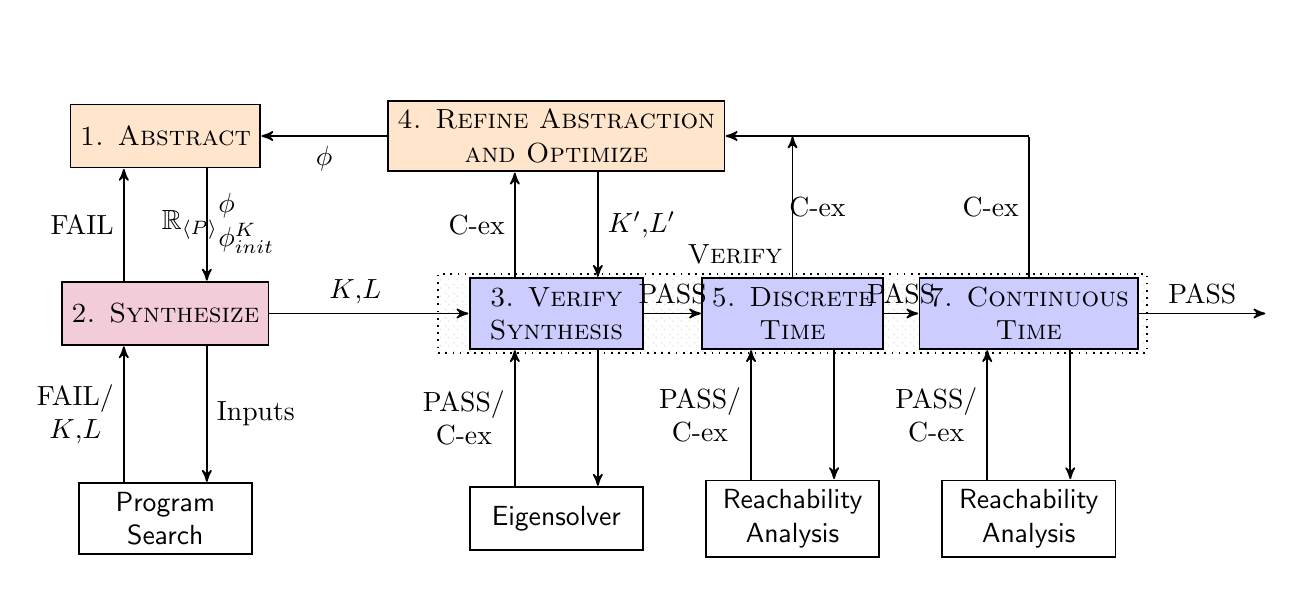
\begin{tikzpicture}[scale=0.3,->,>=stealth',shorten >=.2pt,auto, semithick, initial text=, ampersand replacement=\&,]
  \matrix[nodes={draw, fill=none, shape=rectangle, minimum height=.2cm, minimum width=.2cm, align=center}, row sep=.8cm, column sep=1.5cm] {
  \coordinate (aux1);\&\&
  \coordinate (aux2);
  \coordinate (aux3) at ([xshift=3cm]aux2); \\
  \node[minimum width=2.2cm, minimum height=0.8cm, fill=orange!20] (model1) {{\sc 1. Abstract}};
  \& complexnode/.pic={
    \coordinate (model);
    \node[minimum width=2.2cm, minimum height=0.8cm, fill=orange!20] (model2) at ([xshift=-3cm]model.center) {{\sc 4. Refine Abstraction}\\{\sc and Optimize}};
     \coordinate (model3) at ([xshift=0cm]model.center);
     \coordinate (model4) at ([xshift=3cm]model.center);
   } ;\\
   \node[minimum width=2.2cm, minimum height=0.8cm, fill=purple!20] (synth) {{\sc 2. Synthesize}};
   \&
   complexnode/.pic={ 
     \node[rectangle,draw,dotted,
	minimum width=9cm,
	minimum height=1cm,
        pattern=north west lines, pattern color=gray!20,
	label={\sc Verify~~~~~~~~~~~},] (verif) {};
     \node[minimum width=2.2cm, minimum height=0.8cm, fill=blue!20] (verif1) at ([xshift=-3cm]verif.center) {{\sc 3. Verify}\\{\sc Synthesis}};
     \node[minimum width=2.2cm, minimum height=0.8cm, fill=blue!20] (verif2) at ([xshift=0cm]verif.center) {{\sc 5. Discrete}\\{\sc Time}};
     \node[minimum width=2.2cm, minimum height=0.8cm, fill=blue!20] (verif3) at ([xshift=3cm]verif.center) {{\sc 7. Continuous}\\{\sc Time}};
   } 
   \& \coordinate (done);\\
   \& \\
   \node[minimum width=2.2cm, minimum height=0.8cm] (gp) {{\sf Program}\\{\sf Search}};
   \&
   complexnode/.pic={ 
     \coordinate (aux);
   \node[minimum width=2.2cm, minimum height=0.8cm] (bmc) at ([xshift=-3cm]aux.center) {\sf Eigensolver};
   \node[minimum width=2.2cm, minimum height=0.8cm] (fp)  at ([xshift=0cm]aux.center) {\sf Reachability \\ \sf Analysis};
   \node[minimum width=2.2cm, minimum height=0.8cm] (sv)  at ([xshift=3cm]aux.center) {\sf Reachability \\ \sf Analysis};
   }   
    \\
  };
   \path
    (synth.east) edge node[xshift=-0.5em,align=center] {$\mat{K}$,$\mat{L}$} (verif1.west)
    (verif1.east) edge node {PASS} (verif2.west)
    (verif2.north) edge node[xshift=.8cm] {C-ex} (model3.south)
    (verif2.east) edge node {PASS} (verif3.west)
    (verif3.north) edge[-] node {C-ex} (model4.south)
    %(model2.west) edge node {$k$,$X_0'$} (model2.east)
    (model4.west) edge node {} (model2.east)
    ([xshift=-5em]fp.north) edge node[align=center]  {PASS/\\C-ex} ([xshift=-5em]verif2.south)
    ([xshift=-5em]sv.north) edge node[align=center]  {PASS/\\C-ex} ([xshift=-5em]verif3.south)
    ([xshift=5em]verif1.south) edge node[align=center] {} ([xshift=5em]bmc.north)
    ([xshift=5em]verif2.south) edge node[align=center] {} ([xshift=5em]fp.north)
    ([xshift=5em]verif3.south) edge node[align=center] {} ([xshift=5em]sv.north)
    ([xshift=-5em]bmc.north) edge node[align=center]  {PASS/\\C-ex} ([xshift=-5em]verif1.south)
    (verif3.east) edge node {PASS} (done)
    ([xshift=5em]synth.south) edge node[align=center] {Inputs} ([xshift=5em]gp.north)
    ([xshift=-5em]gp.north) edge node[align=center] {FAIL/\\$\mat{K}$,$\mat{L}$} ([xshift=-5em]synth.south)
   ([xshift=5em]model1.south) edge node[align=center,xshift=-.7cm] {$\mathbb{R}_{\langle P \rangle}$} 
([xshift=5em]synth.north)
   node[align=left,yshift=-0.7cm,xshift=.5cm] {{$\phi$}\\{$\phi_{init}^K$}} %{$\phi_\mathit{safety}$}\\ 
   ([xshift=-5em]synth.north) edge node[align=center] {FAIL} ([xshift=-5em]model1.south);
   \path[->]
    ([xshift=-5em]verif1.north) edge node[align=center]  {C-ex} ([xshift=-5em]model2.south)
    ([xshift=5em]model2.south) edge node[align=center]  {$\mat{K}'$,$\mat{L}'$} ([xshift=5em]verif1.north)
    (model2.west) edge node[align=center] {$\phi$} (model1.east);

   %(verif4.north) edge node[align=center] {} ([xshift=10.5cm]aux2)
   %([xshift=10.5cm]aux2) edge node[align=center] {Increase Sampling Rate} (aux1);

 \end{tikzpicture}
}
\caption{CEGIS-OR: CEGIS with Optimization Refinement. Orange boxes (light) are modelling
stages, blue boxes (dark) are verification stages, and the red box is the synthesis stage.}
\label{fig:CEGIS-OR}
\end{figure}

%-------------------------------
\section{Experimental Evaluation}
\label{exp:evaluation}
%-------------------------------

The benchmark suite employed to evaluate the proposed technique is 
composed by seven models extracted from the control literature~\cite{acrobot,cstr,CHEN1979389,KOKOTOVIC198023,gajic2008optimal,Franklin15,maglev,converters}.
In order to obtain statistically relevant results, we have taken these models
and modified each possible combination of their parameters by a 10\% tolerance,
thus creating seven hundred benchmarks from this base.
In the verification module, we have used the tool Axelerator~\cite{} .


%-------------------------------
\subsection{Results}
\label{exp:results}
%-------------------------------

\begin{table}
\centering
\footnotesize
%
\begin{tabular}{| r | l | c | c | r | r | r | r | r | r | r |}
%
\hline
\# & \multicolumn{1}{|c|}{Benchmark} & \multicolumn{1}{|c|}{order} & \multicolumn{1}{|c|}{Number of} & \multicolumn{3}{|c|}{CEGIS} & \multicolumn{3}{|c|}{CEGIS-OR} \\
   &                                 & & \multicolumn{1}{|c|}{benchmarks}  & \multicolumn{1}{|c|}{Min} & \multicolumn{1}{|c|}{Median} & \multicolumn{1}{|c|}{Max} & \multicolumn{1}{|c|}{Min} & \multicolumn{1}{|c|}{Median} & \multicolumn{1}{|c|}{Max}\\\hline
1  & DC Motor          & 2 & 100 & 9.5\,s & 1.9\,s& \xmark& 1.2\,s &   3.1\,s &   14.1\,s\\
2  & Helicopter        & 3  & 100 & \xmark & \xmark & \xmark & 6.7\,s  &   18.9\,s & \xmark\\
3  & Inverted Pendulum & 4 & 100 &   9.7\,s & \xmark &\xmark & 12.0\,s  &  18.1\,s &  414.0\,s\\
4  & Magnetic Pointer  & 2  & 100 & \xmark & \xmark & \xmark& 4.6\,s  &  39.0\,s &  \xmark \\
%5 & Magnetic Suspension          & 2 & 1 & 12.2\,s& 0.6\,s & & & N/A  &   N/A &   N/A\\
5  & Pendulum          & 2 & 100 & 14.0\,s & 2.0\,s & \xmark&1.2\,s  &   1.5\,s &   4.3\,s\\
6  & Suspension        & 4 & 100 & 73.7\,s& \xmark & \xmark &24.0\,s  &   46.1\,s &  557.9\,s\\
7  & Tape Driver       & 3 & 100 & 10.1\,s& 140.3\,s & \xmark &2.6\,s  &   10.5\,s &   104.6\,s\\
%9 & Satellite          & 2 & 1 & 9.4\,s& 0.7\,s & & & N/A  &   N/A &   N/A\\
%   & Total                 &   & 2002 & & & & & 1.2\,s & 16.1\,s & 876.8\,s\\
\hline
%
\end{tabular}
\vspace{0.05in}
\caption{\label{tab:cegis_results}
Experimental results. Minimum, Maximum and Median times for standard CEGIS vs CEGIS-OR on multiple benchmarks. \xmark~indicates failure to find a controller, either due to timeout or insufficient numeric precision (bitvectors are limited to 64bits).}
\end{table}

Using the described technique we managed to synthesize controllers for X benchmarks, with a median synthesis time of $18.8$ seconds.
%and the maximum observed synthesis time was under 10 minutes for a $4^{th}$ order system ($8^{th}$ order considering the observer).
We consider these times short enough to be of practical use to control engineers.
There are cases for which the system fails to find a controller.  We use a
relatively short timeout, so it is possible longer timeouts would result in a
valid solution. However, as stated before, the solution is sound but incomplete,
so it is impossible to tell if a solution exists in these cases. 

In order to show the improvements due to our optimization-enhanced CEGIS, we
compared our approach against a standard CEGIS procedure.  For the majority of
our benchmarks, we observe that our approach is significantly faster than
standard CEGIS. We further note the cases where standard CEGIS times out, which
represent an improvement of several orders of magnitude for our optimization
approach.  The magnitude of the improvement is largely dependent on the shape
of the problem. 

The smaller benchmarks (order=2) tend to show little or no improvement when we
apply CEGIS-OR.  The reason is that for these benchmarks the synthesis time using
Solution Generalization is already small, and the overhead of the abstraction is
often equal or larger than the gain obtained.

More interesting cases appear when we increase the order, showing initially that
benchmarks that timed-out using standard CEGIS are now running in under 2
minutes using CEGIS-OR. This is the result of removing several multiplications which are
known to be difficult for SAT solvers.  Furthermore, when we introduce Optimization
Refinement there is a further improvement up to an order of magnitude.  This second
improvement is due to the elimination of counterexamples that would have been
created without the refinement. Since further synthesis require increasingly
complex models which are linear in the number of multiplications, eliminating 
these results in large improvements.  In cases when the initial candidate is
suitable, we gain nothing with the refinement and therefore find similar times.
Improvements using this approach will therefore be observed in higher order
systems or when the safety specification is tight and the original loop would
require multiple counterexamples.

%%-------------------------------
%\subsection{Threats to validity}
%\label{exp:threats-to-validity}
%%-------------------------------
%Since our synthesisers use abstract aproximations of the real dynamics, our solution is not complete.
%it is possible to have models where a true solution is not found although it exists.
%Soundness is ensured by the verifiers,but once again, since these use over-approximations of the real dynamics, they may also reject valid solutions, hence affecting completeness. 

%-------------------------------
\section{Conclusions}
\label{sec:conclusions}
%-------------------------------

CEGIS-OR shows promise in exploiting modularity for improved response. 
It however relies on the use of application-specific optimization, 
which requires adequate tools for exploring different types of properties.  
Our results show significant improvement in terms of scalability over standard CEGIS approaches, 
with an ability to explore complex properties, hence many synthesis tasks may be tackled with it. 
In particular we note that our synthesis loop is more efficient for
models where the solution space is formed by connected spaces where
optimization algorithms or localized synthesis are likely to be more
efficiently than global synthesis. 
Finally our application to control synthesis provides a solid proof
of concept for scalable optimal control synthesis of LTI systems. 

There is still a need to extend CEGIS-OR to MIMO models and to analyse more general properties, 
which may also require exploring other optimization methods for control systems. 

\newpage
\bibliographystyle{splncs03}
\bibliography{paper}
\newpage
\appendix

%+++++++++++++++++++++++++++++++++++++++++++++++++++++++++++++++++++++++++++++++
\subsection{Discretization of linear time invariant dynamical systems}\label{sec:continuous_LTI}
%+++++++++++++++++++++++++++++++++++++++++++++++++++++++++++++++++++++++++++++++

Discretization of a continuous dynamical system turns the ODE into a difference
equation, assuming zero-order hold for the input $\vec{u}$ (i.e. the value $u(t)$
 is fixed for the integration period), %and continuous integration for the noise $\vec{w}$, 
into
\begin{align}
\label{eq:discretization}
\vec{x}_{k+1} &= \mat{A}_d\vec{x}_k+\mat{B}_d\vec{u}_k\\% + \vec{w}_k\\
y_k &= \mat{C}_d \vec{x}_ k + \mat{D}_d \vec{u}_ k 
\end{align}
%with covariance for $\vec{w}_k$, $N ( 0 , Q_d )$
where
\begin{align}
\label{eq:discretize}
\mat{A}_d &= e^{\mat{A} T_s} \\%= \mathcal{L}^{-1} { ( s \mat{I} - \mat{A} )^{-1} }_{t = T_s}\\
\mat{B}_d &= \int_{t = 0}^{T_s} e^{\mat{A} t} dt\ \mat{B} = \mat{A}^{-1} ( \mat{A}_d - \mat{I} ) \mat{B}\\
\mat{C}_d &= \mat{C}\\
\mat{D}_d &= \mat{D} %\\
%Q_d &= \int_{t = 0}^{T_s} e^{\mat{A} t} Q e^{\mat{A}^T t} dt
\end{align}
and $T_s$ is the sample time. Then
\begin{align*}
\forall k,  \vec{x}(kT_s)=\vec{x}_k \text{ and } \vec{y}(kT_s) = \vec{y}_k
\end{align*}
%Let $g_d(k)=\mathcal{G}(t,g(t),T)$ be a function that performs the discretization described above, where $g(t)$
%represents the continuous dynamics and $g_d(k)$ the corresponding discrete dynamics. 
%Let $G(s)=\mathcal{L}(g(t))$ and $G_d(z)=\mathcal{Z}(g_d(k))$ be the corresponding Laplace and Z-transforms
%of $g(t)$ and $g_d(k)$. Given this relation, we have 
%$$G_d(z)=G(z)|_{z=e^{sT}} \text{ where } g_d(k)=\mathcal{G}(t,g(t),T) \wedge T < \frac{1}{.5f_s}$$
%Where $.5f_s$ is the Nyquist frequency of $g(t)$. This last restriction is introduced to avoid the effects of aliasing
%which could cause non-existent `phantom' poles to appear otherwise at fractions of the true frequency they represent. 
The eigenvalues of $\vec{A}_d$ %corresponding to the poles of $G_d(z)$,
and those of $\vec{A}$ %corresponding to the poles of $G(s)$
are related as follows:
$\hat{\lambda}_i=e^{\lambda_iT_s} \text{ where } \hat{\lambda}_i \in \sigma(\vec{A}_d) \text{ and } \lambda_i \in \sigma(\vec{A})$
where $\sigma(\cdot)$ is the spectrum of a matrix.
The following remark is worth mentioning regarding the above.
\begin{remark}
The witnessed maximum amplitude of the discrete signals $\vec{x}_k,\vec{y}_k$
may be smaller to that of $\vec{x}(t),\vec{y}(t)$ due to synchronism at
fraction-frequency sampling. This means that safety verification of the state space
must account for this condition.
\end{remark}
Imagine that a signal $\vec{x}(t)=sin\left({\omega_f t}\right)$. If we sample
this signal at intervals $T_s=\frac{\pi}{\omega_f}$ starting at $t=0$, then all
measured samples will be $0$.  For this reason, systems must be sampled at
intervals smaller than the maximum composing frequency of the source signal
$T_s<\frac{\pi}{\omega_max}$.  This is the so called Nyquist Criterion~\cite{Astrom08}.  
The maximum amplitude of the original signal can be upper bounded from the
observed values using the inverse cosine of the sampling function.
Since equation \eqref{eq:discretization} models \eqref{eq:dynamical} \note{fix ref}, we may use the semantics defined in Section
\ref{sec:model_semantics} to analyse continuous dynamical systems.

%+++++++++++++++++++++++++++++++++++++++++++++++++++++++++++++++++++++++++++++++
\section{Numeric representations and soundness} \label{sec:numeric_rep}
%+++++++++++++++++++++++++++++++++++++++++++++++++++++++++++++++++++++++++++++++

In embedded software programs interacting and/or simulating physical plants it
is of great importance to understand the effects of the chosen numeric
representation for the continuous state-space. 
These representations are almost invariably approximations to the original which
are assumed to be precise enough as to not cause any trouble, but it is precisely
this assumption that often results in the most difficult and dangerous errors.
There are generally speaking two paradigms for representing numbers in programs:
fixed and variable precision numbers.  We refer to both of these as finite word
length representations (FWL).  In fact, these subdivide into multiple data types
such as integer bit-vectors, fixed or floating point numbers and rationals). In 
this section we will be discussing fixed and floating point numbers.
On one hand, we have variable word length types which will attempt to use as
much memory as needed to precisely represent the original domain (usually the
reals). In this case the limitations are caused by memory and speed, both of
which are directly affected by the increasingly larger word lengths. Multiple
Precision Floating Point Arithmetic and Software Rationals are good examples of
these cases. It is possible for some of these data types to have memory
constraints, at which point they fall into the second category.
Fixed precision data types are most common in software programs. Whether
they be Floating Point or Fixed Point (of which integers are the special case
for 0 decimal places) numbers, the problem arises in the misrepresentation of
the reals (or equivalent data type being represented).
Let $\mathbb{R}_{\langle M,F \rangle}$ be a fixed point domain with $M$ bits
representing the binary word length of the representation and $F$ bits
representing the pre-scaling $2^{-F}$ (\emph{i.e} the number of bits after
the decimal place).  We note that a negative $F$ denotes an integer
multiplication that adds $-F$ trailing zeros in the number represented by
$M$.
Let also $\mathbb{R}_{\langle M,[E] \rangle}$ be a floating point
domain with $M$ bits mantissa and $E$ bits exponent.  This domain
corresponds to $$\mathbb{R}_{\langle M,[E] \rangle} = \bigcup_F
\mathbb{R}_{\langle M,F \rangle} \text{ where } F \in [-2^{E-1}, ...\,,2^{E-1}]$$ This
definition important because it means that the distance between any two
numbers in the domain depends on the location of those numbers.  Since we
have shown that a floating point domain is a union of a number of fixed
point domains, we will continue our reasoning on fixed point only, which
will apply to the floating point domain by extension.  Operations on these
numbers will incur errors that can be bound
by~\cite{DBLP:conf/arith/BrainTRW15}.  We examine the most relevant ones:
%
\begin{enumerate}
\item Truncation\\
Let $\mathcal{F}_{\langle M,F \rangle} : \mathbb{R} \rightarrow \mathbb{R}_{\langle M,F \rangle}$
be a truncation function, defined as:
\begin{align*}
x_{\langle M,F \rangle}=\mathcal{F}_{\langle M,F \rangle}(x) = x-\delta \text{ where } \delta=mod_F(x, x_{\langle M,F \rangle})
\end{align*} 
where $mod_F(\cdot)$ is the modulus operation performed on the last bit of the representation ($2^{-F}$).\\
The number $\delta$ corresponds to the truncation error of the representation and it will propagate across operations.
\item Rounding\\
Every time an operation is performed on a number in the $\mathbb{R}_{\langle M,F \rangle}$ domain, an error may be
introduced due to truncation of the result. 
The following errors appear in simple operations:
\begin{enumerate}
\item Addition/Subtraction
\begin{align*}
&x_{\langle M,F_1\rangle} \pm y_{\langle M,F_2\rangle}=z_{\langle M,F\rangle} + \delta,  F=\text{min}(F_1,F_2)\\
&\text{ where } |\delta| \leq 2^{-F} \text{ and } F_1=F_2 \Rightarrow \delta=0.
\end{align*}
\item Multiplication
\begin{align*}
&x_{\langle M,F_1\rangle} * y_{\langle M,F_2\rangle}=z_{\langle M,F\rangle} + \delta, \text{ where } F=F_1+F_2 \text{ and } |\delta| \leq 2^{-F}
\end{align*}
%\item Division\\
%The operations performed by our controllers in the FWL
%domain do not include division.  However, we do use division in computations
%at the precision of the plant.  Here the error depends on whether the
%divisor is greater or smaller than the dividend:  $x_{\langle M,F_1\rangle} / y_{\langle M,F_2 \rangle} = c_3 + \delta_{T3}$
%where $\delta_{T3}$ is $(\delta_{T2}\cdot x - \delta_{T1}\cdot y)/(\delta_{T2}^2 - \delta_{T2} y)$,
\end{enumerate}
We note here that not all systems truncate equally.  In the
definition above $\delta$ may be positive or negative, and even this
decision can be made dependent on the sign of $x$.  Common cases in computer
systems are: round downwards (\emph{ie} to $-\infty$), round upwards
(\emph{ie} to $+\infty$), and round to zero.  Rounding errors are cumulative
which means the overall error will statistically increase with every
operation, thus single transition algorithms can be more precise in this
respect than iterative ones because they perform fewer operations needing
rounding.
\item Overflow\\
Another source of error introduced by FWL representations is that of overflow.
The finite word length set a maximum representable number in the domain
$\pm \overline{M} \text{ where }  \overline{M}=2^{M-F}-2^{-F}$, which means that any number
outside this range cannot be accurately represented by the domain (\emph{eg} $\delta=x-\overline{M}$).
In the case of floating point, a special cases for infinity has been introduced, which addresses
some of these issues, but once the error has gone to infinity, the numbers become meaningless.
It is the responsibility of software designers and tools to account for overflows and either
supply saturation functions to prevent them or raise alarms in their presence. In the case
of verification, the latter is seen as a safety problem.
\item Null/Zeno behaviour\\
Whilst this work does not explore Zeno behaviours, it is worth noting that this
effect may be caused by rounding errors in floating point programs. The reason for this
is that if an operation contains two numbers which belong to disjoint sub-domains
(\emph{ie} neither number can be represented in the domain of its counterpart), the
resulting operation may become a no-op/skip, subsequently destabilizing the program.
\end{enumerate}

We will use the domain $\mathbb{R}_{\langle C \rangle} \text{ where } \langle C \rangle = \langle M_c,F_c \rangle$
to represent a digital implementation of LTI dynamics which we will refer to as the controller, and 
$\mathbb{R}_{\langle P \rangle} \supseteq \mathbb{R}_{\langle C \rangle}$
to represent the domain of a digital model of the dynamics of a real plant when evaluated by a verification tool.
Furthermore, we will refer to the errors incurred by the calculations performed in these domains as finite word length (FWL) effects. 

%+++++++++++++++++++++++++++++++++++++++++++++++++++++++++++++++++++++++++++++++
\subsection{Modeling quantization as noise} \label{sec:quantization-noise}
%+++++++++++++++++++++++++++++++++++++++++++++++++++++++++++++++++++++++++++++++
In Figure \ref{fig:observersystem2} we introduced
several sources of noise, which are due to quantization effects. We now describe
their nature and create a sound model for them to be used during our synthesis
and verification process.

%Let us first consider the effect of the quantization errors. 
%Within the controller, state values are manipulated at low precision.
%Furthermore, the quantizers for the DAC and the ADC introduce truncation errors
%which we denote by the effect of the functions $\mathcal{F}_{\langle D \rangle}$
%and $\mathcal{F}_{\langle A \rangle}$, respectively. Finally, let us call $\vec{\nu}_e$ the
%error caused by the FWL effects on the observer
%\todo{the observer was not defined..}
%(\emph{i.e} the numerical errors 
%in the calculations as opposed to the estimation error).
%The inputs are computed using the following equation: 
%%
%\begin{align}
%u_{k}&=\mathcal{F}_{\langle D \rangle}\left(-\mat{K}_{\langle C \rangle}\cdot\left(\mathcal{F}_{\langle C \rangle}\left(\mathcal{F}_{\langle A \rangle}(\vec{x}_{k})\right)\right) +\vec{\nu}_e\right)
%\label{eq:uk}
%\end{align}
%
%This induces two types of the errors: first, the truncation
%error due to the domain transformations $\mathcal{F}_{\langle *
%\rangle}(\cdot)$; and second, the rounding error introduced by the
%multiplication operation.  We represent these errors as non-deterministic
%additive noise.

During any given ADC conversion, the continuous signal will be sampled in
the real domain and transformed by $\mathcal{F}_{\langle A \rangle}
(x)$. This sampling uses a threshold which is defined by the
less significant bit ($q_{a}=2^{-F_a}$) 
of the ADC and some non-linearities of the circuitry.  The overall conversion is
%
$$\vec{y}_k=\mathcal{F}_{\langle A \rangle}\left(y(kT_s)\right), \text{ with }  \vec{y}_k \in \left[y(kT_s)-\frac{q_{a}}{2}, y(kT_s)+\frac{q_{a}}{2}\right] \,.$$
%
where $t = kT_s$, and $T_s$ is the sampling time and $k$ the current iteration of the loop.
If we denote the error in the conversion by $\nu_k=y_k-y(t)$, then we may define
some bounds for it $\nu_k \in [-\frac{q_{a}}{2}, \frac{q_{a}}{2}]$.

We will assume, for the purposes of this analysis, that the domain of the
ADC is that of the digital controller (i.e, the quantizer includes a digital
gain added in the code resulting in $\mathbb{R}_{\langle A \rangle}=\mathbb{R}_{\langle C \rangle}$).
The process of quantization in the DAC is
similar except that it is calculating $\mathcal{F}_{\langle D\rangle}
(\mathcal{F}_{\langle C \rangle} (x)) $.  If these domains
are the same ($\mathbb{R}_{\langle D \rangle}=\mathbb{R}_{\langle C \rangle}$), or if the DAC
resolution in higher than the ADCs ($\mathbb{R}_{\langle D \rangle}\supseteq\mathbb{R}_{\langle C \rangle}$), then the DAC quantization error is equal
to zero.  From the above equations we can now define the ADC and DAC
quantization noises ${\nu_1}_k \in [-\frac{q_a}{2}, \frac{q_a}{2}]$ and
${\nu_2}_k \in [-\frac{q_d}{2}, \frac{q_d}{2}]$, where given the above assumptions $q_d=q_a=q_c$. 
This is illustrated in Figure \ref{fig:observersystem2} where $Q_1$ is the quantizer of the ADC
and $Q_2$ the quantizer for the DAC.  These bounds hold irrespective of
whether the noise is correlated, hence we may use them to over-approximate
the noise effect on the state space progression over time.  The
resulting dynamics are
%
\begin{align*}
%\label{eq:pre_quantization}
\vec{x}_{k+1} = \mat{A}_d\vec{x}_k+\mat{B}_d({u}_k+{{\nu}_2}_k), \quad u_k = -\mat{K}\vec{x}_{k}+{{\nu}_1}_k, 
\end{align*}
%
which result in the following closed-loop dynamics:
%
\begin{align*}
%\label{eq:quantization}
\vec{x}_{k+1} &= (\mat{A}_d-\mat{B}_d\mat{K}_d) \vec{x}_k+\mat{B}_d{{\nu}_2}_k +{{\nu}_1}_k \,. 
\end{align*}

%+++++++++++++++++++++++++++++++++++++++++++++++++++++++++++++++
\subsection{Round-off errors}
\label{sec:roundoff-noise}
%+++++++++++++++++++++++++++++++++++++++++++++++++++++++++++++++

Let $q_*=2^{-F_*}$ be the smallest difference
between two numbers in their corresponding domains.  Assuming that our
system truncates numbers to the nearest value, this means that the error
$\delta$ introduced by the function $\mathcal{F}_{\langle * \rangle}$ is
$\delta_*=\mathcal{F}_{\langle * \rangle}(x)-x \in \left[-\frac{q_*}{2}, 
\frac{q_*}{2}\right]$.
We note that in the case of floating point,the
choice of $F_*$ is taken from the largest multiplication found (e.g.,
$\norm{\mat{A}}_1\norm{\vec{x}}_1, \text{ where }  \vec{x} \models \phi_\mathit{safety}$,
where $\phi_\mathit{safety}$ is defined in \ref{eq:safetyspec}). From these
equations we can define:
%
\begin{align*}
\nu_1 \in \left[-\frac{q_a}{2}, \frac{q_a}{2}\right] \cap  \left[-\frac{q_c}{2}, \frac{q_c}{2}\right],
\nu_2 \in \left[-\frac{q_d}{2}, \frac{q_d}{2}\right]
\end{align*}

We may also bound $\nu_2'$ as follows:
\begin{align*}
\delta\left(\mat{K}_{\langle C\rangle} \vec{x}_{\langle C\rangle} \right) &\in \left[ -p \frac{q_c}{2},\, p \frac{q_c}{2}\right]\\
{\vec{\nu_e}}_i &\in \left[ -(p+2) \frac{q_c}{2}, (p+2) \frac{q_c}{2}\right], i \in [1, ...\,,p]\\
\Rightarrow \nu_2' &\in \left[  -p(\norm{\mat{K}_{\langle C \rangle}}_1+2) \frac{q_c}{2},\, p(\norm{\mat{K}_{\langle C \rangle}}_1+2) \frac{q_c}{2}\right]
\end{align*}
Similarly we also find
\begin{align*}
\nu_1' &\in \left[  -p(\norm{{\mat{C}_d}_{\langle C \rangle}}_1+2) \frac{q_c}{2},\, p(\norm{{\mat{C}_d}_{\langle C \rangle}}_1+2) \frac{q_c}{2}\right]
\end{align*}
The proof derives from $\norm{\mat{K}\vec{x}}_1 \leq \norm{\mat{K}}_1\norm{\vec{x}}_1$.

%+++++++++++++++++++++++++++++++++++++++++++++++++++++++++++++++++++++++++++++++
\section{Control theory} \label{sec:control_theory}
%+++++++++++++++++++++++++++++++++++++++++++++++++++++++++++++++++++++++++++++++

The semantics discussed in sections \ref{sec:model} do not describe all
properties of interest in our systems.  In some cases, specific values or
substructures define hidden properties which can only be inferred given an
appropriate transformation.  Since our models are being applied to linear
control systems, and in particular to feedback systems with observers, we
provide a summary of the important elements using control theory for their
transformations.

A feedback system is one where the output is fed back into the input, thus
making part or all of the system a closed system (i.e. no inputs).
Such a system is exemplified in figure \ref{fig:sampledsystem}.  Since the
feedback line creates a loop in the diagram this is known as a closed loop,
and the overall behaviour of the resulting system is said to have closed loop dynamics.
The feedback may be direct or have further transformations, some of which will
be discussed in this section.  For the moment we will also point out that in the
models we are interested in, this feedback is digital and thus creates some
further considerations regarding discretization.

The objective of the feedback is to adhere to some properties we decide to control.
In most cases these properties include stability.  We define stability as the ability of
the system output to remain bounded given a bounded input. This is known as BIBO
stability. Further constraints to this property may be added to enforce stronger stability 
(e.g. convergent).  We discuss the requirements we are interested in in the following.
%+++++++++++++++++++++++++++++++++++++++++++++++++++++++++++++++++++++++++++++++
\subsection{Static output feedback and pole placement} \label{sec:pole_place}
%+++++++++++++++++++++++++++++++++++++++++++++++++++++++++++++++++++++++++++++++

\begin{figure*}[htb]
\centering

\tikzset{add/.style n args={4}{
    minimum width=6mm,
    path picture={
        \draw[circle] 
            (path picture bounding box.south east) -- (path picture bounding box.north west)
            (path picture bounding box.south west) -- (path picture bounding box.north east);
        \node[draw=none] at ($(path picture bounding box.south)+(0,0.13)$)     {\small #1};
        \node[draw=none] at ($(path picture bounding box.west)+(0.13,0)$)      {\small #2};
        \node[draw=none] at ($(path picture bounding box.north)+(0,-0.13)$)    {\small #3};
        \node[draw=none] at ($(path picture bounding box.east)+(-0.13,0)$)     {\small #4};
        }
    }
 }

\resizebox{1.0\textwidth}{!}{
 \begin{tikzpicture}[scale=0.6,-,>=stealth',shorten >=.2pt,auto,
     semithick, initial text=, ampersand replacement=\&,]

  \matrix[nodes={draw, fill=none, shape=rectangle, minimum height=.2cm, minimum width=.2cm, align=center}, row sep=.6cm, column sep=.6cm] {
    \node[draw=none] (r) {$R(z)$};
%   \& \coordinate (aux0);
   \& \node[circle,add={-}{+}{}{}] (circle) {};
   \node[draw=none] (ez) at ([xshift=1cm,yshift=.15cm]circle)  {$e(z)$};
   \& \node[rectangle,draw,
	minimum width=1cm,
	minimum height=1cm,
        label=\textbf{Controller}] (cz) {{\sc C(z)}};
   \node[draw=none] (ud) at ([xshift=1cm,yshift=.15cm]cz)  {$U(z)$};
     
   \& complexnode/.pic={ 
      \node[rectangle,draw,
	minimum width=3cm,
	minimum height=1.6cm,
	label=\textbf{DAC},] (dac) {};
     \node[circle,add={}{+}{+}{},fill=gray!20] (q2) at ([xshift=-.65cm]dac.center) {};
     \node[draw=none] (q2t)  at ([xshift=-.65cm,yshift=-.65cm]dac.center) {{\sc Q2}};
     \node[draw=none] (v2)  at ([xshift=-.65cm,yshift=1.5cm]dac.center) {$\nu_2(z)$};
     \node[fill=gray!20] (zoh) at ([xshift=.65cm]dac.center) {{\sc ZOH}};}   
   \& \node[rectangle,draw,
	minimum width=1cm,
	minimum height=1cm,
        label=\textbf{Plant}] (gs) {{\sc $G(s)$}};
   \node[draw=none] (ud) at ([xshift=-2cm,yshift=.15cm]gs)  {$U(s)$};
   \node[draw=none] (y) at ([xshift=2cm,yshift=.15cm]gs)  {$Y(s)$};
   \& complexnode/.pic={ 
     \node[rectangle,draw,
	minimum width=4cm,
	minimum height=1.6cm,
	label=\textbf{ADC},] (adc) {};
   \draw[] ([xshift=-1cm]adc.center) -- ++(0.5,0.2cm);
   \coordinate (switch1) at ([xshift=-1cm]adc.center);
   \coordinate (switch2) at ([xshift=-0.4cm]adc.center);
   \node[circle,add={}{+}{+}{},fill=gray!20] (q1) at ([xshift=1cm]adc.center) {};} 
     \node[draw=none] (q2t)  at ([xshift=1cm,yshift=-.65cm]adc.center) {{\sc Q1}};
   \node[draw=none] (v1)  at ([xshift=1cm,yshift=1.5cm]adc.center) {$\nu_1(z)$};
   \& \coordinate (aux1);
   \& \node[draw=none] (yz) {$Y(z)$};\\
   \& \coordinate (aux3); 
   \&
   \&
   \& 
   \& 
   \& \coordinate (aux2);\\
  };


  \path[->] (v1) edge (q1.north);
  \path[->] (v2) edge (q2.north);
  \path[->] (r) edge (circle.west);
  \path[->] (aux1) edge (yz);
  \path  
   (circle.east) edge (cz)
   (cz.east) edge (q2.west)
   (q2.east) edge (zoh.west)
   (zoh.east) edge (gs.west)
   (switch2) edge (q1.west)
   (q1.east) edge (aux1.west)
   (gs.east) edge (switch1.west)
   (aux1.south) edge (aux2.north)
   (aux2.west) edge (aux3.east); 
  \path[->]  (aux3.north) edge (circle.south);
 \end{tikzpicture}
}
 \caption{Closed loop digital control system\label{fig:sampledsystem}}
\end{figure*}

Given an unstable plant with divergent dynamics, the problem of stabilizing the
output is to find a controller that results in convergent closed loop dynamics.
The term Static Output Feedback relates to the desired effect of having a static
output given a fixed reference signal.  In modern embedded systems, said
controller is a digital program, which means that the closed loop dynamics are
subject to time and space discretization as described in
sections~\ref{sec:continuous_LTI} and~\ref{sec:numeric_rep}.
In real a physical plant, these discretizations are performed by an
Analog-to-Digital Converter(ADC) which samples the output of the plant at
intervals $T_s$ (time discretization) and quantizes it to an FWL representation
(space discretization).  Conversely, a Digital-to-Analog Converter(DAC)
transforms a discretized value into a real input to the physical plant.
In general terms, when analysing such systems, the controller is known to have
discrete dynamics, whereas the plant must be discretised based on the sample
and hold characteristics. The ADC/DAC converters are considered to introduce a
quantization noise on the system as shown in Figure~\ref{fig:sampledsystem}.
Let the quantizer~$Q1$ be the source of a non-deterministic noise~$\nu_{1}$
and~$Q2$ be the source of a non-deterministic noise~$\nu_{2}$.
Convergence of such a system is a frequency domain property, which is why we
first analyse the system using its transfer function.  The transfer function of
a system relates its input and output in the frequency domain (more generally
in the Laplace domain for continuous time systems and the Z-domain for discrete
time).  In the case of linear systems, these correspond to the characteristic
polynomials of the system dynamics (i.e. the polynomial whose roots are the
eigenvalues of the dynamics). The following equation models the system,
encompassing the discretization of the plant:
%
\begin{equation}
Y(z)=C(z)G(z)(R(z)-Y(z))+\nu_{1}(z)+\nu_{2}(z)C(z)G(z),
\end{equation}
%
The above can be rewritten as follows:
%
\begin{equation}
\label{eq:outputfunctions}
Y(z)=H_1(z)R(z)+H_2(z)\nu_{1}(z)+H_3(z)\nu_{2}(z),
\end{equation}
%
where
%
\begin{align}
H_1(z)=\frac{C(z)G(z)}{1+C(z)G(z)},\\
H_2(z)=\frac{1}{1+C(z)G(z)},\\
H_3(z)=\frac{G(z)}{1+C(z)G(z)}.
\end{align}
%

\begin{assumption}
\label{whitenoise}
%
The quantization noises $\nu_{1}$ (from $Q1$) and $\nu_{2}$ (from $Q2$) are
uncorrelated white noises and their amplitudes are always bounded by the
half of quantization step~\cite{astrom1997computer}, i.e., $\vert \nu_{1}
\vert \leq \frac{q_{1}}{2}$ and $\vert \nu_{2} \vert \leq \frac{q_{2}}{2}$,
where $q_{1}$ and $q_{2}$, respectively, are the quantization steps of ADC
and DAC.
% 
\end{assumption}

It is known that a discrete-time linear system is said to be Bounded-Input and Bounded-Output
(BIBO) stable if and only if every pole of its transfer function lies inside
the unit circle \cite{Astrom08}.  Analyzing Eq.~\eqref{eq:outputfunctions}, the following
proposition states necessary conditions for BIBO stability of the closed-loop system
in Figure~\ref{fig:sampledsystem}, since the exogenous signals $R(z)$,
$\nu_{1}$, and $\nu_{2}$ are bounded. Hence, our close loop system is stable if the poles in
$H_1(z) , H_2(z) $ and $H_3(z)$ are inside the unit circle. Since all three transfer functions share the same poles,
we only need to look at the roots of the polynomial
$$C_n(z)G_n(z)+C_d(z)G_d(z) : C(z)=\frac{C_n(z)}{C_d(z)} \wedge G(z)=\frac{G_n(z)}{G_d(z)}$$
Any controller that ensures these roots lie within the unit circle is a stabilizing controller for the system.

This same analysis can be applied to MIMO systems where there is a transfer functions of the system
for each combination of input-output. Rather than examine the transfer functions of these systems, we will first
look at minimal descriptions of the state space dynamics that will help us extract them with little extra effort whilst 
providing us with tools to analyse other properties.

%+++++++++++++++++++++++++++++++++++++++++++++++++++++++++++++++++++++++++++++++
\subsection{Controllable canonical form} \label{sec:reachable}
%+++++++++++++++++++++++++++++++++++++++++++++++++++++++++++++++++++++++++++++++

Let us have a discrete time Single Input Single Output (SISO) system with a $p^{th},q^{th}$ order model with $p\geq q$.
$$y[k]=\sum_{i=1}^p a_{p-i}y[k-i]+\sum_{i=0}^{q-1} b_{p-i}u[k-i],$$
where $y$ is the output of the system and $u$ its input.
The equivalent LTI dynamics of such a model are:
\begin{align}
\label{eq:cf_SISO}
\vec{x}_{k+1}=&\mat{A}_c\vec{x}_k+\mat{B}_cu_k, \text{ where } \vec{x}_k=[\begin{array}{cccc}y_k&y_{k-1}&\hdots&y_{k-(p-1)}\end{array}]^T\\
y_k=&\mat{C}_c\vec{x}_k + b_0u_k\nonumber\\
\mat{A}_c=&\left[
\begin{array}{ccccc}
-a_{p-1}&-a_{p-2}&\cdots&-a_1&-a_0\\
1&0&0&\cdots&0\\
0&1&0&\cdots&0\\
\vdots&\ddots&\ddots&\ddots&\vdots\\
0&\cdots&0&1&0
\end{array}\right],
\mat{B}_c=\left[
\begin{array}{c}
1\\0\\ \vdots\\ 0\\ 0
\end{array}\right]\nonumber\\
\mat{C}_c=&[\begin{array}{ccccc}b_0-a_0b_p&b_1-a_1b_p&\cdots&b_{p-1}-a_{p-1}b_p\end{array}] \text{ where } b_i=0 \text{ and } i \in [0, ...\,,p-q]\nonumber
\end{align}

where the coefficients $a_i$ describe the characteristic polynomial of the system. This matrix shape is
called a Controllable Canonical Form because the dynamics of the feedback are directly related to these
coefficients. Specifically, given a feedback controller $\mat{K}_c$ for any particular system, the closed loop dynamics
are
\begin{align}
\vec{x}_{k+1}=(\mat{A}-\mat{B}\mat{K})\vec{x}_k
\label{eq:closeloopdynamics}
\end{align}
which translated to Reachable Canonical Form will have the shape
\begin{align}
\mat{A}_c-\mat{B}_c\mat{K}_c=&\left[
\begin{array}{ccccc}
k_{n-1}-a_{n-1}&k_{n-2}-a_{n-2}&\cdots&k_1-a_1&k_0-a_0\\
1&0&0&\cdots&0\\
0&1&0&\cdots&0\\
\vdots&\ddots&\ddots&\ddots&\vdots\\
0&0&\cdots&1&0
\end{array}\right]
\label{eq:cf_SISO_fb}
\end{align}
which means we can directly modify each coefficient by selecting a controller parameter.
In the MIMO case, the Controllable Canonical Form has the following shape:
\begin{align}
\mat{A}_c=&\left[
\begin{array}{ccccc}
-\mat{a}_{p-1}\mat{M}_{p-1}&-\mat{a}_{p-2}\mat{M}_{p-2}&\cdots&-\mat{a}_{2}\mat{M}_{2}&-\mat{a}_0\mat{M}_0\\
\mat{I}_{n-1}&0&0&\cdots&0\\
0&\mat{I}_{n-2}&0&\cdots&0\\
\vdots&\ddots&\ddots&\ddots&\vdots\\
0&0&\cdots&\mat{I}_0&0
\end{array}\right],
\mat{B}_c=\left[
\begin{array}{c}
\mat{M}_0\\0\\ \vdots\\ 0\\ 0
\end{array}\right]\nonumber\\
\mat{C}_c=&[\begin{array}{ccccc}\mat{\Gamma}_{0}&\mat{\Gamma}_{1}&\cdots&\mat{\Gamma}_{p-1}\end{array}] 
\label{eq:cf_MIMO}
\end{align}
with $\mat{I}_i,\mat{M}_i \in \mathbb{R}^{q_i \times q_i}, \mat{a}_i \in \mathbb{R}^{q \times q_i}, \mat{\Gamma}_i \in \mathbb{R}^o \text{ and for }  i \in [0, ...\,,p-q], \mat{\Gamma}_{i}=0$, where $q$ is the number of inputs, $q_i$ the number of inputs with a transfer function of order of at least $i$, $\mat{I}_i$ an identity matrix, $\mat{M}_i$ an upper triangular matrix with 1s in its diagonal, $\mat{a_i}$ a matrix of coefficients of the $i^{th}$ order on its diagonal, and $o$ the number of outputs. Ideally, $\forall i>0, \mat{M}_i=\mat{I}_i$

Any LTI system can be transformed into a controllable canonical form by a matrix $\mat{T}_c$ such that $\vec{x}=\mat{T}_c\hat{\vec{x}}$
Then the dynamics of the controllable form are
\begin{align}
\hat{\vec{x}}_{k+1}=&\mat{A}_c\hat{\vec{x}}_k+\mat{B}_cu_k, \text{ where } \mat{A}_c=\mat{T}_c\mat{A}\mat{T}_c^{-1} \text{ and } \mat{B}_c=\mat{T}_c\mat{B}\\
y_k=&\mat{C}_c\hat{\vec{x}}_k + b_0u_k, \text{ where } \mat{C}_c=\mat{C}\mat{T}_c^{-1}\nonumber
\end{align}
where $\mat{T}_c$ can be calculated as follows:

Let 
\begin{equation}
\mat{R}=[\begin{array}{ccccc}\mat{B}&\mat{A}\mat{B}&\mat{A}^2\mat{B}&\hdots&\mat{A}^{p-1}\mat{B}\end{array}]
\label{eq:rncf}
\end{equation}
be the reachability matrix of the system, and
\begin{equation}
\mat{R}_{c}=\left[\begin{array}{ccccc}1&a_{p-1}&a_{p-2}&\hdots&a_1\\0&1&a_{p-1}&\hdots&a_2\\ \vdots&\ddots&\ddots&\ddots&\ddots\end{array}\right]
\label{eq:rcf}
\end{equation}
the reachability matrix of the canonical form. Then 
\begin{equation}
\mat{T}_c=\mat{R}_{c}\mat{R}^{-1}
\label{eq:to_cf}
\end{equation}

%-------------------------------
\subsection{Stability of a controlled system} 
\label{sec:closed_stability}
%-------------------------------
There are a number of algorithms that can be
used for stability analysis~\cite{daes20161,Bessa16}.

A discrete-time LTI system as \eqref{eq:closeloopdynamics} is
asymptotically stable if all the roots of its characteristic
polynomial (i.e., the eigenvalues of the closed-loop matrix $A_d - B_d
K$) are inside the unity circle of the complex plane, i.e., their
absolute values are strictly less than one~\cite{astrom1997computer}
(this simple sufficient condition can be generalised, however this is
not necessary in our work).  In this work, we express this stability
specification $\phi_\mathit{stability}$ in terms of a check known as
\emph{Jury's criterion}~\cite{fadali}: this is an easy algebraic
formula to select the entries of matrix $K$ so that the closed-loop
dynamics are shaped as desired.

Since the canonical forms used in this work use the coefficients of the
characteristic polynomial $S(z)$ as opposed to its roots (which are
comparatively hard to calculate for a SAT solver due to the number of
multiplications involved), we choose Jury's criterion~\cite{astrom1997computer}
to check the stability in the~$Z$-domain in view of its efficiency.

We~consider the following form for $S(z)$:
%
\begin{equation*}
S(z) = z^{p}+a_1z^{p-1}+\cdots+a_{p-1}z+a_p.
\end{equation*}

and build the matrix
$\mat{M} \in \mathbb{R}^{p \times p}$ from its coefficients such that:
%
\begin{align*}
\mat{M}_{1,j}&=a_j\\
\mat{M}_{i+1,j}&=\left\{
\begin{array}{ll}
0,&j>p'\\
\mat{M}_{i,j}-\mat{M}_{i,p'-j+1}\frac{\mat{M}_{i,1}}{\mat{M}_{i,p'}} &j\leq p'
\end{array}
\right.\\
p'&=p-i+1
\end{align*}
%
$S(z)$ is the characteristic polynomial of a stable system if and
only if the following conditions hold~\cite{astrom1997computer}:
\begin{align*}
\phi_\mathit{stability}(S) \equiv
(S(1) > 0) \wedge ((-1)^p S(-1) > 0) \wedge (|a_p| < 1) \wedge \bigwedge\limits_{i=1}^p (\mat{M}_{i,1} > 0).
\end{align*}

%+++++++++++++++++++++++++++++++++++++++++++++++++++++++++++++++++++++++++++++++
\subsection{Observable canonical form} \label{sec:observable}
%+++++++++++++++++++++++++++++++++++++++++++++++++++++++++++++++++++++++++++++++
In most real implementations, the internal state of a plant cannot be
directly measured but rather inferred from its effect on the output by
using an observer.  Essentially, a state observer is a system that
provides an estimate of the internal state of a given real system,
from measurements of the input and output of the real system.
This means that contrary to a stateless reactive controller, an observer
controller has memory of the states (i.e. it is stateful).

Take for example a system where we are given the position of a robot
arm in a single axis.  Our objective is to move the arm to pick an object 
from a known location along that axis.  The input of the robotic arm is an
acceleration.  The position of the arm will vary depending on the speed, which
in turn varies with the acceleration.  However, if we do not know the speed, we
will not be able to reach our target smoothly.  An observer for this design could
simply calculate the speed by keeping a memory (state) of the previous position
and calculate the difference with the current position in the given time interval.

A closed-loop digital control system with observer is shown in Figure~\ref{fig:observersystem}.
Note that the variables of a state observer are denoted by a "$~\hat{}~$" (e.g. {$\hat {\vec{x}}(k)$})
to distinguish them from the variables of the actual physical system.
Moreover, $\vec{y}_e=\hat{\vec{y}_k}-\vec{y}_k$ is the output estimation error defined
as the difference between the real output $\vec{y}_k$ and estimated one $\hat{\vec{y}_k}$, whereas
$\mat{L}$ is the error sensitivity matrix, which amplifies the output estimation error.
The figure also contains references to $\nu_1$, $\nu_2$, $\nu_1'$, $\nu_2'$ and $\nu_t$, which
denote noise and will be explained later in the dissertation.
Lastly, $k_r$ is a reference gain required by the model.

Presuming a sampled model of the plant as described in \eqref{eq:discretize}, the dynamics of the observer are:
\begin{equation}
\label{eq:to_of}
\hat{\vec{x}}_{k+1}=({\mat{A}_d}_{\langle C \rangle}-\mat{L}{\mat{C}_d}_{\langle C \rangle})\hat{\vec{x}}_k+{\mat{B}_d}_{\langle C \rangle}\vec{u}+\mat{L}\vec{y}
\end{equation}
where the subindex ${\langle C \rangle}$ represents the domain of the controller $\mathbb{R}_{\langle C \rangle}$ such that ${\mat{A}_{\langle C \rangle}=\mathcal{F}_{\langle C \rangle}(\mat{A}_d)}$, ${\mat{B}_{\langle C \rangle}=\mathcal{F}_{\langle C \rangle}(\mat{B}_d)}$ and ${\mat{C}_{\langle C \rangle}=\mathcal{F}_{\langle C \rangle}(\mat{C}_d)}$.
The differentiation between $\mat{*}_{\langle C \rangle}$ and $\mat{*}$ will be exploited later in this work. For the time being we will assume they are the same. 
%is an observer of the system $\vec{x}_{k+1}=\mat{A}\vec{x}+\mat{B}\vec{u} : \vec{y}=\mat{C}\vec{x}$. 
%$p_i$ are user selected values which will affect the error of the observer estimator. 
Since the feedback of this system depends on $\mat{C}$ rather than $\mat{B}$, the Reachable
Canonical form is no longer suitable. Hence we require an Observable Canonical Form.
For SISO systems, this is:
\begin{align}
\label{of_SISO}
\mat{A}_o=&\left[
\begin{array}{cccccc}
-a_{p-1}&1&0&0&\cdots&0\\
-a_{p-2}&0&1&0&\cdots&0\\
-a_{p-3}&0&0&1&\cdots&0\\
\vdots&\vdots&\ddots&\ddots&\ddots&\vdots\\
-a_0&0&0&0&\cdots&1
\end{array}\right],
\mat{B}_o=\left[
\begin{array}{c}
\Gamma_{p-1}\\ \Gamma_{p-2}\\ \vdots\\ \Gamma_0
\end{array}\right]\\
\mat{C}_o=&[\begin{array}{cccccc}\ \ \ \ 1&\ \ \ \ 0&0&0&\cdots&0\end{array}] \nonumber
\end{align}

We notice here that $\mat{A}_o=\mat{A}_c^T, \mat{C}_o=\mat{B}_c^T$
and $\mat{B}_o=\mat{C}_c^T$, which also applies to the MIMO case.

Let 
\begin{equation}
\label{eq:wnof}
\mat{W}=\left[\begin{array}{c}\mat{C}\\ \mat{C}\mat{A}\\ \mat{C}\mat{A}^2\\ \vdots\\ \mat{C}\mat{A}^{p-1}\end{array}\right]
\end{equation}
be the observability matrix of the system, and
\begin{equation}
\label{eq:wof}
\mat{W}_{o}=\mat{R}_{c}^{-1}
\end{equation}
the observability matrix of the canonical form (see eg~\cite{Astrom08}). Then the matrix $\mat{T}_o=\mat{W}^{-1}\mat{W}_{o}$ will transform an observable system into its canonical form.
For simplicity of the description, we aggregate the noises as follows:
$\eta_1=\nu_1+\nu_1'+\nu_t$ and $\eta_2=\nu_2+\nu_2'$,
where $\nu_1$ and $\nu_2$ are the quantization noises introduced by the ADC and the DAC, $\nu_t$ is the noise introduced by the delay, and $\nu_1'$ and $\nu_2'$ are quantization noises caused by roundoffs in the FWL operations (see Section~\ref{sec:quantization-noise}).
Assuming that the observer dynamics are an exact copy of the real ones, ($\mat{*}_{\langle C \rangle}=\mat{*}$), the closed loop dynamics of this system are given by:
\begin{align}
\left [\begin{array}{c}\vec{x}\\ \vec{x}_e \end{array}\right]_{k+1}
=\left [\begin{array}{cc}\mat{A}_d-\mat{B}_d\mat{K}&\mat{B}_d\mat{K}\\ \mat{0}&\mat{A}_d-\mat{L}\mat{C}_d\end{array}\right]
\left [\begin{array}{c}\vec{x}\\ \vec{x}_e \end{array}\right]_k
+\left [\begin{array}{cc}\mat{B}_dk_r&\mat{0}\\ \mat{0}&-\mat{L}\end{array}\right]\left [\begin{array}{c}\vec{r}_k+\vec{\eta}_2\\ \vec{\eta}_1\end{array}\right]
\label{eq:observer_LTI}
\end{align}
where $\vec{x}_e=\vec{x}-\hat{\vec{x}}$ is the estimation error of the state space by the observer.
Note that this matrix is not in canonical form. A transformation using both reachability and observability matrices is required. This is achieved as follows:
By translating the coordinate system to 
\begin{equation}
\left[\begin{array}{c}\vec{x}'\\ \vec{x}_e'\end{array}\right]=
\left[\begin{array}{cc}\mat{T}_c & \mat{0}\\\mat{0} & \mat{T}_o\end{array}\right]
\left[\begin{array}{c}\vec{x}\\ \vec{x}_e\end{array}\right]
\end{equation}
where $\mat{T}_c=\mat{R}_{c}\mat{R}^{-1}$ and $\mat{T}_o=\mat{W}^{-1}\mat{W}_{o}$, we can transform equation \eqref{eq:observer_LTI} into the equivalent canonical form
\begin{align}
\left [\begin{array}{c}\vec{x}'\\ \vec{x}_e' \end{array}\right]_{k+1}
=& \left [\begin{array}{cc}\mat{A}_{c}&\mat{B}_{o}\\ \mat{0}&\mat{A}_{o}\end{array}\right]
\left [\begin{array}{c}\vec{x}'\\ \vec{x}_e' \end{array}\right]_k
+\left[\begin{array}{cc}\mat{T}_c\mat{B}_d&\mat{0}\\\mat{0}&-\mat{T}_o\mat{L}\end{array}\right]\left [\begin{array}{c}\mat{k}_r\vec{r}_k+\vec{\eta}_2\\ \vec{\eta}_1\end{array}\right]\nonumber\\
\vec{y}_k
=& \mat{C}_{t}\vec{x}_k% + \mat{D}_{d}\vec{u}_k
\label{eq:observer_LTI_cf}
\end{align}
where
{
\begin{align*}
\mat{A}_{c}=&\mat{T}_c\left(\mat{A}_d-\mat{B}_d\mat{K}\right)\mat{T}_c^{-1}&
\mat{A}_{o}=&\mat{T}_o\left(\mat{A}_d-\mat{L}\mat{C}_d\right)\mat{T}_o^{-1}\\
\mat{B}_{o}=&\mat{T}_c\mat{B}_d\mat{K}\mat{T}_o^{-1}&
\mat{C}_t=&\mat{C}_d\mat{T}_c
\end{align*}
Replacing the matrices in \eqref{eq:observer_LTI_cf} with appropriate symbols:
\begin{align}
\mat{A}'=&\left [\begin{array}{cc}\mat{A}_{c}&\mat{B}_{o}\\ \mat{0}&\mat{A}_{o}\end{array}\right]&
\mat{B}'=&\left[\begin{array}{cc}\mat{T}_c\mat{B}_d&\mat{0}\\\mat{0}&-\mat{T}_o\mat{L}\end{array}\right]
\label{eq:of_dynamics}
\end{align}
}
we get
\begin{displaymath}
\tilde{\vec{x}}_{k+1}=\mat{A}' \tilde{\vec{x}}_{k}+\mat{B}' \tilde{\vec{u}}_k \text{ where }
\tilde{\vec{x}}_k=\left [\begin{array}{c}\vec{x}'\\ \vec{x}_e' \end{array}\right]_k \text{ and }
\tilde{\vec{u}}_k=\left [\begin{array}{c}\vec{r}_k+\vec{\eta}_2\\ \vec{\eta}_1\end{array}\right]
\label{eq:simple_observer_LTI}
\end{displaymath}
This has a similar structure to \eqref{eq:discretization} which will be helpful in our analysis.

\begin{figure*}[htb]
\centering
\tikzset{add/.style n args={4}{
    minimum width=6mm,
    path picture={
        \draw[circle] 
            (path picture bounding box.south east) -- (path picture bounding box.north west)
            (path picture bounding box.south west) -- (path picture bounding box.north east);
        \node[draw=none] at ($(path picture bounding box.south)+(0,0.13)$)     {\small #1};
        \node[draw=none] at ($(path picture bounding box.west)+(0.13,0)$)      {\small #2};
        \node[draw=none] at ($(path picture bounding box.north)+(0,-0.13)$)    {\small #3};
        \node[draw=none] at ($(path picture bounding box.east)+(-0.13,0)$)     {\small #4};
        }
    }
 }

\resizebox{1.0\textwidth}{!}{
 \begin{tikzpicture}[scale=0.6,-,>=stealth',shorten >=.2pt,auto,
     semithick, initial text=, ampersand replacement=\&,]

  \matrix[nodes={draw, fill=none, shape=rectangle, minimum height=.2cm, minimum width=.2cm, align=center}, row sep=.6cm, column sep=.6cm] {
    \node[draw=none] (r) {$r_k$};
    \node[rectangle,draw,
	minimum width=1cm,
	minimum height=1cm,] (gain)at ([xshift=1.2cm]r) {\sc $k_r$};
    
   \& \node[circle,add={-}{+}{+}{}] (circle) {};
   \node[draw=none] (ez) at ([xshift=1cm,yshift=.15cm]circle)  {$u_k$};
   \node[draw=none] (v2p)  at ([yshift=1.2cm]circle) {$\nu_2'$};
   \node[rectangle,draw,minimum width=1cm,minimum height=1cm] (Kd) at ([xshift=0,yshift=-5.5cm]circle)  {\sc $\mat{K}_{\langle C \rangle}$};
   \coordinate (kdsouth) at ([yshift=-3cm]Kd);
   
      
   
   \& complexnode/.pic={ 
      \node[rectangle,dashed,draw,minimum width=3cm,minimum height=1.6cm,label=\textbf{DAC}] (dac) {};
     \node[circle,add={+}{+}{}{},fill=gray!20] (q2) at ([xshift=-.65cm]dac.center) {};
     \node[draw=none] (q2t)  at ([yshift=.55cm]q2) {{\sc Q2}};
     \node[draw=none] (v2)  at ([yshift=-1.5cm]q2) {$\nu_2$};
     \node[fill=gray!20] (zoh) at ([xshift=.65cm]dac.center) {\sc ZOH};
   }   

   \& complexnode/.pic={ 
      \node[rectangle,dashed,draw,minimum width=8cm,minimum height=3.5cm,label=\textbf{Continuous Plant}] (plant)  at ([yshift=-.5cm]dac.center) {};
      \node[rectangle,draw,minimum width=1cm,minimum height=1cm] (B) at ([xshift=-2.5cm,yshift=.5cm]plant.center)  {\sc $\mat{B}$};
      \node[draw=none] (u) at ([xshift=-1cm,yshift=.15cm]B)  {$u(t)$};
      \node[circle,add={+}{+}{}{}] (p1) at ([xshift=-1.3cm,yshift=.5cm]plant.center) {};
      \node[draw=none] (xdot) at ([xshift=.85cm,yshift=.15cm]p1)  {$\dot{\vec{x}}(t)$};   
      \node[rectangle,draw,minimum width=1cm] (int) at ([xshift=.5cm,yshift=.5cm]plant.center) {\sc $\int$};
      \coordinate (xsouth) at ([xshift=1cm]int);
      \node[draw=none] (x) at ([xshift=1cm,yshift=.15cm]int)  {$\vec{x}(t)$};   
      \node[rectangle,draw,minimum width=1cm,minimum height=1cm] (C) at ([xshift=2.7cm,yshift=.5cm]plant.center)  {\sc $\mat{C}$};
      \node[draw=none] (y) at ([xshift=1cm,yshift=.15cm]C)  {$\vec{y}(t)$};   
      \node[rectangle,draw,minimum width=1cm,minimum height=1cm] (A) at ([xshift=.5cm,yshift=-1cm]plant.center)  {\sc $\mat{A}$};
      \coordinate (aeast) at ([xshift=1cm]A);
      \coordinate (awest) at ([xshift=-1.8cm]A);
    }   
    \node[circle,add={+}{+}{}{}]at ([xshift=2cm]C) (lag) {};
    \node[draw=none] (vt)  at ([yshift=-1.5cm]lag) {$\nu_t$};
   complexnode/.pic={ 
      \node[rectangle,dashed,draw,minimum width=8cm,minimum height=5cm,label=\textbf{Discrete Observer}] (observer)  at ([yshift=-5cm]plant.center) {};
      \node[rectangle,draw,minimum width=1cm,minimum height=1cm] (Bd) at ([xshift=-2.5cm]observer.center)  {\sc ${\mat{B}_d}_{\langle C \rangle}$};
      \node[draw=none] (ud) at ([xshift=-1cm,yshift=.15cm]Bd)  {$u_k$};
      \node[circle,add={+}{+}{+}{}] (o1) at ([xshift=-1.3cm]observer.center) {};
      \node[draw=none] (xd) at ([xshift=.85cm,yshift=.15cm]o1)  {$\hat{\vec{x}}_{k+1}$};   
      \node[rectangle,draw,minimum width=1cm] (delay) at ([xshift=.5cm]observer.center) {\sc $z^{-1}$};
      \coordinate (xdsouth) at ([xshift=1.3cm]delay);
      \coordinate (fbsouth) at ([xshift=1.3cm,yshift=-3cm]delay);
      \node[draw=none] (xdp) at ([xshift=1cm,yshift=.15cm]delay)  {$\hat{\vec{x}}_k$};   
      \node[rectangle,draw,minimum width=1cm,minimum height=1cm] (Cd) at ([xshift=2.7cm]observer.center)  {\sc ${\mat{C}_d}_{\langle C \rangle}$};
      \node[draw=none] (y) at ([xshift=.4cm,yshift=.8cm]Cd)  {$\hat{\vec{y}}_k$};   
      \node[rectangle,draw,minimum width=1cm,minimum height=1cm] (Ad) at ([xshift=.5cm,yshift=-1.5cm]observer.center)  {\sc ${\mat{A}_d}_{\langle C \rangle}$};
      \coordinate (adeast) at ([xshift=1.3cm]Ad);
      \coordinate (adwest) at ([xshift=-1.8cm]Ad);
      \node[circle,add={-}{}{+}{+}] (o2) at ([xshift=2.7cm,yshift=1.5cm]observer.center) {};
      \node[draw=none] (v1p) at ([yshift=1.2cm]o2) {$\nu_1'$};
      \node[rectangle,draw,minimum width=1cm,minimum height=1cm] (Ld) at ([xshift=.5cm,yshift=1.5cm]observer.center)  {\sc $\mat{L}_{\langle C \rangle}$};
      \coordinate (ldwest) at ([xshift=-1.8cm]Ld);
      \coordinate (bdwest) at ([xshift=-5.5cm]Bd);
      \coordinate (uksouth) at ([xshift=-5.5cm,yshift=5.5cm]Bd);
      \coordinate (o2east) at ([xshift=7.17cm]o2);
    }   
    
   \& complexnode/.pic={ 
     \node[rectangle,dashed,draw,minimum width=3.5cm,minimum height=1.6cm,label=\textbf{ADC},] (adc) {};
     \draw[] ([xshift=-1cm]adc.center) -- ++(0.5,0.2cm);
     \coordinate (switch1) at ([xshift=-1cm]adc.center);
     \coordinate (switch2) at ([xshift=-0.4cm]adc.center);
     \node[circle,add={+}{+}{}{},fill=gray!20] (q1) at ([xshift=.6cm]adc.center) {};
     \node[draw=none] (q2t)  at ([yshift=.55cm]q1) {\sc Q1};
     \node[draw=none] (v1)  at ([yshift=-1.5cm]q1) {$\nu_1$};
     \node[draw=none] (y) at ([xshift=.85cm,yshift=.15cm]q1)  {$\vec{y}_k$};       
     \coordinate (ykeast) at ([xshift=1.9cm]q1);
   } 
   \& \coordinate (aux1);
   \& \\
  };

  \path[->] (v1) edge (q1.south);
  \path[->] (v2) edge (q2.south);
  \path[->] (vt) edge (lag.south);
  \path[->] (v1p) edge (o2.north);
  \path[->] (v2p) edge (circle.north);
  \path[->] (r) edge (gain.west);
  \path[->] (gain.east) edge (circle.west);
  \path[->] (circle.east) edge (q2.west);
  \path       (q2.east) edge (zoh.west);
  \path[->] (zoh.east) edge (B.west);
  \path
   (B.east) edge (p1.west)
   (p1.east) edge (int.west)
   (xsouth) edge (aeast)
   (aeast) edge (A.east)
   (A.west) edge (awest)
   (awest) edge (p1.south)
   (int.east) edge (C.west)
   (C.east) edge (lag.west)
   (lag.east) edge (switch1.west)
   (switch2) edge (q1.west);
  \path
   (q1.east) edge (ykeast)
   (ykeast) edge (o2east);
  \path       (uksouth) edge (bdwest);
  \path[->] (bdwest) edge (Bd.west);
  \path
   (Bd.east) edge (o1.west)
   (o1.east) edge (delay.west)
   (xdsouth) edge (adeast)
   (adeast) edge (Ad.east)
   (Ad.west) edge (adwest)
   (adwest) edge (o1.south)
   (o2.west) edge node {$\vec{y}_e$} (Ld.east)
   (Ld.west) edge (ldwest)
   (ldwest) edge (o1.north)
   (delay.east) edge (Cd.west)
   (Cd.north) edge (o2.south)
   (o2east) edge (o2.east)
   (xdsouth) edge (fbsouth)
   (fbsouth) edge (kdsouth);
  \path[->]  (kdsouth) edge (Kd.south);
  \path[->] (Kd.north) edge (circle.south);
 \end{tikzpicture}
}
 \caption{Closed-loop digital control system with observer\label{fig:observersystem}}
\end{figure*}

%+++++++++++++++++++++++++++++++++++++++++++++++++++++++++++++++++++++++++++++++
\subsection{Stability of an observed system}\label{sec:cof_stability}
%+++++++++++++++++++++++++++++++++++++++++++++++++++++++++++++++++++++++++++++++

Careful examination of the matrices of the observed system\eqref{eq:of_dynamics} reveals that because $\mat{A}'$ is
upper block diagonal, the spectrum of $\mat{A}'$ is equal to the union of
the spectrum of $\mat{A}_{c}$ and $\mat{A}_{o}$, which can be calculated
separately.  In other words, the characteristic polynomial of the closed loop is
equal to the multiplication of the characteristic polynomials of the controller closed loop
and the observer error when seen independently.
%
\begin{align*}
P(z)=P_K(z)P_L(z)=\left(z^p+\sum_{i=0}^{p-1}{(a_i-k_i)z^{i}}\right) \left(z^p+\sum_{i=0}^{p-1}{(a_i-l_i)z^{i}}\right)
\end{align*}

We get the stability specification by applying Jury's Criterion to these polynomials.

%For a stabilised closed loop, we need these roots to remain within the unit circle (left hand side of the plane for continuous time).
%Whilst this is not a sufficient condition for verifying safety properties, it is a necessary one, therefore we will review this verification process.
%The direct approach would be to calculate the roots of the polynomials (\emph{ie} the eigenvalues of the matrix), but this ends up being to costly, particularly in the case of synthesis, so we use an indirect method.
%
%Jury's criteria is a mathematical method used to verify whether the roots of the polynomial are within the unit circle by exploring solely the coefficients of the polynomial. In order to achieve this, we first create a matrix $\mat{M} \in \mathbb{R}^{(n+1) \times (n+1)}$ with zero-indexed coefficients $m_{i,j} : i,j \in [0,, ...\,,n]$ in the following form:
%
%\begin{equation}
%\left[\begin{array}{ccccc}
%c_0&c_1&\hdots&c_{n-1}&c_n\\
%m_{\scriptscriptstyle 0,0}-m_{\scriptscriptstyle 0,n}^*\frac{m_{0,n}^*}{m_{0,0}}&m_{\scriptscriptstyle 0,1}-m_{\scriptscriptstyle 0,n-1}^*\frac{m_{0,n}^*}{m_{0,0}}&\hdots&m_{\scriptscriptstyle 0,n-1}-m_{\scriptscriptstyle 0,1}^*\frac{m_{0,n}^*}{m_{0,0}}&0\\
%\vdots&\vdots&\vdots&\vdots&\vdots\\
%m_{\scriptscriptstyle i-1,0}-m_{\scriptscriptstyle i-1,n-i+1-j}^*\frac{m_{i-1,n-i+1}^*}{m_{i-1,0}}&m_{\scriptscriptstyle i-1,1}-m_{\scriptscriptstyle i-1,n-i+1-j}^*\frac{m_{i-1,n-i+1}^*}{m_{i-1,0}}&\hdots&0&0\\
%m_{\scriptscriptstyle n-1,0}-m_{\scriptscriptstyle n-1,1-j}^*\frac{m_{n-1,1}^*}{m_{n-1,0}}&0&\hdots&0&0\\
%\end{array}\right]
%\end{equation}
%
%The first row corresponds to the coefficients of the original polynomial. Notice also that every row has a polynomial one degree lower than the previous. The sufficient and necessary conditions for the polynomial in row 0 to have all of its roots inside the unit circle are~\cite{}:
%\begin{align}
%|c_n|<c_0&&
%\sum_{i=0}^n c_i > 0&&
%(-1)^n\sum_{i=0}^n c_i (-1)^{n-i}> 0&&
%m_{i,0}>0
%\end{align}
%
%Notice that in both our polynomials $c_0=1$ and we only use reals.

%-------------------------------
\section{Proofs of theorems \label{sec:proofs}}
%-------------------------------
\setcounter{theorem}{0}
\setcounter{corollary}{0}
 %+++++++++++++++++++++++++++++++++++++++++++++++++++++++++++++++++++++++++++++++
 \subsubsection{Accelerated dynamics for continuous time models without inputs}\label{sec:cont_acc_no_inputs}
 %+++++++++++++++++++++++++++++++++++++++++++++++++++++++++++++++++++++++++++++++
 Given a specific time $T$, the state $\vec{x}(t=T)$ can be expressed as a linear function of $\vec{x}_0$ as described below.
 
 \begin{theorem}
 Given $\dot{\vec{x}}(t)=\mat{A}\vec{x}(t)$, where $\mat{A}=\mat{S}\mat{J}\mat{S}^{-1}$, we have
 \begin{align}
 \vec{x}_T&=\vec{x}(t=T)=\mat{A}_{T}\vec{x}_0\\
 \mat{A}_{T}&= \mat{S}
 \left [ \begin{array}{cccc}
 e^{T\lambda_1}  & s_1\frac{T^{1}e^{T\lambda_i}}{(2)!} & \hdots  & s_i\frac{T^{p-1}e^{T\lambda_i}}{(p-i)!} \\
0 & e^{T\lambda_i}  & s_i\frac{T^{j-i}e^{T\lambda_i}}{(j-i)!} & \vdots \\
\vdots & & \ddots & \vdots \\
0 & \cdots & 0  &e^{T\lambda_i} \\
\end{array} \right ]
 \mat{S}^{-1}
 \label{eq:continuous_tube_dyn}\\
 &\text{where } s_i=\left\{\begin{array}{cc}1&gm(\lambda_i)>1\\0&gm(\lambda_i)=1\end{array}\right.,\nonumber
 \end{align}
$\lambda_i \in \mat{J}$ are the eigenvalues of $\mat{A}$, and $gm(\lambda_i)$ is the geometric multiplicity of $\lambda_i$.  
$\vec{x}_T$ is the state of the system $\dot{\vec{x}}(t)=\mat{A}\vec{x}(t)$ at time t=T.
 \end{theorem}
  If $\mat{J}$ is diagonal and there exists a discrete dynamics matrix for a sampling time $T_d$ such that $A_d=e^{\mat{A} T_d}$, then $\vec{x}_T=A_d^{\frac{T}{T_d}}\vec{x} \text{ with } T \in \mathbb{R}^+$ is the state of the system at time $t=T$.
 \begin{proof}
 Let us recall equation \ref{eq:discretize}. The discrete representation of the system dynamics discretised with sample time $T_1$ is ruled by the formula
 $\mat{A}_1 = e^{\mat{A} T_1}$. From matrix theory, we have 
\begin{align}
 e^{\mat{A}}&=\sum_{k=0}^\infty \frac{1}{k!}\mat{A}^k
\end{align} 
\begin{align} 
 e^{\mat{S}\mat{J}\mat{S}^{-1}}&=\sum_{k=0}^\infty \frac{1}{k!}\left(\mat{S}\mat{J}\mat{S}^{-1}\right)^k
 =\mat{S} \left (\sum_{k=0}^\infty \frac{1}{k!}\mat{J}^k\right) \mat{S}^{-1}\nonumber\\
 &=\mat{S}e^{\mat{J}}\mat{S}^{-1}
\end{align} 
\begin{equation}
\mat{A}=\mat{S}\mat{J}\mat{S}^{-1} \Rightarrow \vec{A}_1 = \mat{S}\mat{J}_1\mat{S}^{-1}= \mat{S}e^{\mat{J} T_1}\mat{S}^{-1}.
 \end{equation}
 
 Let $\mat{J}$ be a diagonal matrix, such that 
 $${\lambda_1}_i=e^{\lambda_i T_1}, \forall \lambda_i \in \mat{J}.$$
 Let us now take a different sample rate $T_2$, such that 
 $${\lambda_2}_i=e^{\lambda_i T_2}, \forall \lambda_i \in \mat{J}.$$
 We can then say that 
 \begin{equation}
 {\lambda_2}_i=e^{\lambda_i T_1 \frac{T_2}{T_1}}={\lambda_1}_i^{\frac{T_2}{T_1}} \Rightarrow A_2=A_1^{\frac{T_2}{T_1}}.
 \end{equation}
 This proves the theorem for $gm(\lambda_i)=1$.
 We now note that given an exponentiated Jordan form with geometric multiplicity, the upper diagonal terms can be
 referenced to the original eigenvalues modified by the sampling rate.
  Let $\mat{J}\in \mathbb{R}^{p \times p}$ be a Jordan Canonical matrix whose powers are described in Equation \eqref{jord:pow}
 Then
\begin{align}
 \mat{J}_1&=\sum_{k=0}^\infty \frac{1}{k!}\left(\mat{J}T_1\right)^k\nonumber\\
 &=\sum_{k=0}^\infty \frac{1}{k!} \left [ \begin{array}{cccc}
 \lambda_i^k  & \binom{k}{1}  \lambda^{k-1} & \hdots  & \binom{k}{p-1} \lambda_i^{k-p+1} \\
& \lambda_i^k  & \binom{k}{1}  \lambda_i^{k-1} & \vdots \\
\vdots & \ddots & \ddots & \vdots \\
& &  &\lambda_i^k \\
\end{array} \right ] T_1^k
\end{align}
The eigenvalues remain the same as in the diagonal case, but the upper triangular terms are of the form:
\begin{align}
\forall j>i, c_{ij}&=\sum_{k=j-i}^\infty \frac{1}{k!}\binom{k}{j-i} \lambda_i^{k-(j-i)}T_1^k\\
&=\frac{1}{(j-i)!}\sum_{k=j-i}^\infty \frac{1}{(k-(j-i))!} \lambda_i^{k-(j-i)}T_1^k\nonumber\\
&=\frac{T_1^{j-i}e^{\lambda_i T_1}}{(j-i)!}\nonumber
\end{align}
which completes the proof for $gm(\lambda_i)>1$. \qed
\end{proof}

 %+++++++++++++++++++++++++++++++++++++++++++++++++++++++++++++++++++++++++++++++
 \subsubsection{Accelerated dynamics for continuous time models with parametric inputs}\label{sec:cont_acc_param_inputs}
 %+++++++++++++++++++++++++++++++++++++++++++++++++++++++++++++++++++++++++++++++
\begin{theorem}
The expression
 \begin{align}
 \vec{x}_T&=\vec{x}(t=T)=\mat{A}^{-1}\vec{x}_T'\nonumber\\
\vec{x}_T'&=\mat{A}\mat{A}_T\vec{x}_0 + (\mat{I}-\mat{A}_T)\mat{B}\vec{u} \text{ where } \forall t \leq T,\ \vec{u}(t)=\vec{u} 
 \end{align}
 with $\mat{A}_T$ as per \eqref{eq:continuous_tube_dyn} is the state of the system $\dot{\vec{x}}(t)=\mat{A}\vec{x}(t)+\mat{B}\vec{u}(t)$ at time $T$ given a parametric input $\vec{u}$.
 \end{theorem}
 \begin{corollary}
 If $\mat{J}$ is diagonal and there exists a discrete dynamics matrix for a sampling time $T_d$ such that $A_d=e^{\mat{A} T_d}$, then $\vec{x}_T=A_d^{\frac{T}{T_d}}\vec{x}+(\mat{I}-\mat{A}_d^{\frac{T}{T_d}}\mat{B}\vec{u}) \text{ with } k \in \mathbb{R}^+$ is the state of the system at time $kT_d$.
 \end{corollary}
 \begin{proof}
 We begin by expanding the equation
 \begin{align}
 \vec{x}_T&=\mat{A}^{-1}\vec{x}_T'\nonumber\\
 &=\mat{A}_T\vec{x}_0 + \mat{A}^{-1}(\mat{I}-\mat{A}_T)\mat{B}\vec{u}\nonumber\\
 &= \mat{A}_T\vec{x}_0 + \mat{B}_T\vec{u}
 \end{align}
 where $\mat{A}_T=e^{\mat{A}T}$ and $\mat{B}_T=\mat{A}^{-1}(\mat{I}-\mat{A}_T)\mat{B}$ correspond to $\mat{A}_d$ and $\mat{B}_d$ in equation \eqref{eq:discretize}
 \end{proof}
  
 %+++++++++++++++++++++++++++++++++++++++++++++++++++++++++++++++++++++++++++++++
 \subsubsection{Accelerated dynamics for continuous time models with discrete time feedback inputs}\label{asec:real_discrete_feedback_inputs}
 %+++++++++++++++++++++++++++++++++++++++++++++++++++++++++++++++++++++++++++++++

The final case we analyse here is that of hybrid time systems, where the
plant dynamics evolve in continuous time while the feedback dynamics evolve
in discrete time.

\begin{theorem}
The expression
 \begin{align}
 \vec{x}_{T} &= (\mat{A}_{T-kT_s}-\mat{B}_{T-kT_s}\mat{K}) (\mat{A}_d-\mat{B}_d\mat{K})^k\vec{x}_0
 \label{eq:cyber_feedback}
 \end{align}
 with $\mat{A}_T, \mat{B}_T$ as per \eqref{eq:continuous_tube_dyn} and $\mat{A}_d, \mat{B}_d$ as per equation \eqref{eq:discretize} is a witness of the system
 \begin{align}
 \dot{\vec{x}}({t}) &= \mat{A}\vec{x}+\mat{B}\vec{u}(t)\nonumber\\
 \vec{u}(t)&=\mat{K}\vec{x}_k, \text{ where }  kT_s \leq t < (k+1)T_s
 \end{align}
 \end{theorem}

\begin{proof}
Let $\mat{K}$ be a feedback controller such that $\vec{u}_k=-\mat{K}\vec{x}_k$ at time $t=kT_s$. Let the output of
the feedback system be a zero order holder such that $\vec{u}(t'+kT_s)=\vec{u}(kT_s), \text{ for }  0 \leq t' < T_s$.
The closed loop dynamics of the system between times $kT_s$ and $kT_s+T_s$ are
\begin{equation}
\vec{x}_{k,t'}=\mat{A}_{t'}\vec{x}_k-\mat{B}_{t'}\mat{K}\vec{x}_k = (\mat{A}_{t'}-\mat{B}_{t'}\mat{K})\vec{x}_k, \text{ where }  0 \leq t' < T_s
\end{equation}
We further explore the dynamics across discrete time boundaries. Let $\mat{A}_d=\mat{A}_{T_s}$ and $\mat{B}_d=\mat{B}_{T_s}$
\begin{align}
\vec{x}_{k}&=\vec{x}_{k-1,T_s}= (\mat{A}_d-\mat{B}_d\mat{K})\vec{x}_{k-1}\\
\vec{x}_{k,T_s} &= (\mat{A}_d-\mat{B}_d\mat{K}) (\mat{A}_d-\mat{B}_d\mat{K})\vec{x}_{k-1}
\end{align}
which accelerating results and setting $T=kT_s+t'$ becomes
\begin{align}
\label{eq:feedback_sampled_cont}
\vec{x}_{k} &= (\mat{A}_d-\mat{B}_d\mat{K}) ^k\vec{x}_0\\
\vec{x}_{T} &= (\mat{A}_{T-kT_s}-\mat{B}_{T-kT_s}\mat{K}) (\mat{A}_d-\mat{B}_d\mat{K})^k\vec{x}_0
\label{eq:feedback_cont}
\end{align}
\end{proof}

%+++++++++++++++++++++++++++++++++++++++++++++++++++++++++++++++++++++++++++++++
\subsubsection{Time delay on discrete time feedback systems} \label{sec:delay}
%+++++++++++++++++++++++++++++++++++++++++++++++++++++++++++++++++++++++++++++++
\begin{theorem}
The error introduced by a delay $t_d$ in the control output $\vec{u}_k$ of a discrete feedback controller for a continuous LTI system can be modelled as a non-deterministic noise signal upper bound by 
\begin{align}
\norm{\vec{y}_{k}-{\vec{y}_{t_d}}_{k}}_1 \leq q_t, \text{ where } q_t=&(\norm{\mat{C}(\mat{B}_{T_s}-\mat{B}_{t_s})}_1+\norm{\mat{C}\mat{A}_{t_s}\mat{B}_{t_d}}_1)\norm{U}_1
\end{align}
where $\vec{y}_{t_d}$ is the output of the system with delay $t_d$, and $\norm{\vec{x}}_1=\sum_{i=0}^{size(\vec{x})} |\vec{x}_i|$ is the $l_1$ norm (in for sets, $\norm{X}_1 = sup \{\norm{\vec{x}}_1 \mid \vec{x} \in X\}$). 
\end{theorem}

\begin{proof}
Let us look at equations \eqref{eq:feedback_sampled_cont} and
\eqref{eq:feedback_cont}.  When we introduce an arbitrary delay $T_d$ where
$t_d=T_d$ and $t_s=T_s-T_d$ we obtain:
%
\begin{align}
\vec{x}_{k} &=\mat{A}_{t_s}(\mat{A}_{t_d}\vec{x}_{k-1}-\mat{B}_{t_d}\mat{K}\vec{x}_{k-2})-\mat{B}\mat{K}\vec{x}_{k-1}\nonumber\\
&=  (\mat{A}_{T_s}-\mat{B}_{t_s}\mat{K})\vec{x}_{k-1}-\mat{A}_{t_s}\mat{B}_{t_d}\mat{K}\vec{x}_{k-2}
\label{eq:delay_cont}
\end{align}
%
Differentiating with the expected progression without delay, we get a delay
error:
%
\begin{align}
{\vec{x}_e}_{k}=&(\mat{B}_{T_s}-\mat{B}_{t_s})\mat{K}\vec{x}_{k-1}-\mat{A}_{t_s}\mat{B}_{t_d}\mat{K}\vec{x}_{k-2}\nonumber\\
=&(\mat{B}_{T_s}-\mat{B}_{t_s})\vec{u}_{k}-\mat{A}_{t_s}\mat{B}_{t_d}\vec{u}_{k-1}
\end{align}
Rather than explicitly calculate this error, we will find an upper bound. Let $U = \bigcup \vec{u}_k$. Propagating the error to the output $\vec{y}_k$ we have:
\begin{align}
{\vec{y}_e}_{k} \subseteq &\mat{C}(\mat{B}_{T_s}-\mat{B}_{t_s})U\oplus\mat{C}\mat{A}_{t_s}\mat{B}_{t_d}U\\
\Rightarrow \norm{{\vec{y}_e}_{k}}_1 \leq & (\norm{\mat{C}(\mat{B}_{T_s}-\mat{B}_{t_s})}_1+\norm{\mat{C}\mat{A}_{t_s}\mat{B}_{t_d}}_1)\norm{U}_1
\end{align}
\end{proof}
We over-approximate the effects of this vector by introducing a noise signal at the output $\nu_t=[-q_t, q_t]$ and use the dynamics of the system without delay.

%-------------------------------
\subsection{Transient response} 
\label{sec:transientspecificationproof}
%-------------------------------
\begin{theorem}
Given a set of eigenvalues for a discrete time model of an $p^{th}$ order system $\lambda_i =e^{\omega_i}, i \in [1, ...\,,p]$, the settling time of the system is upper-bounded by
\begin{equation}
t_s<-log_{\overline{\lambda}}({P_s}), \text{ where }  \overline{\lambda} = \max(|\lambda_i|) \text{ and } \overline{\lambda}<1,\ \forall i \in [1, ...\,,p]
\label{eq:set_time}
\end{equation}
where $0\leq P_s \leq 1$ is the desired percentage of the target within which the output must remain after $t_s$.
\end{theorem}
\begin{proof}
In a SISO system, there are two values that typically define the
response-time of the system (using a step response).
%
\begin{enumerate}
\item The \emph{rise time} is defined as the time it takes the output to reach a percentage (eg $90\%$) of the target value given a step chnage in the input.
\item The \emph{settling time} is defined as the time it takes the output to stabilize within a margin of the target value (eg $10\%$).
\end{enumerate} 
%
In the case of first and second order systems, the decay is governed by the equations 
%
\begin{align*}
&y_{decay}=
&\left\{
\begin{array}{cc}
e^{-|\omega| t}& 1^{st} order\\
e^{\zeta |\omega| t}\left(\frac{\sin\left(|\omega| t\sqrt{1-\zeta^2}+\sin^{-1}\sqrt{1-\zeta^2}\right)}{\sqrt{1-\zeta^2}} \right)&\zeta<1\\
e^{-|\omega| t}-|\omega| t e^{-|\omega| t}&\zeta=1\\
\frac{|\omega| e^{-|\omega_2| t}-|\omega_2| e^{-|\omega| t}}{|\omega|-|\omega_2|}&\zeta>1\end{array}\right.
\end{align*}
where $|\omega|$ and $|\omega_2|$ are the magnitudes of the eigenvalues (roots) of the system and  $\zeta=-\cos(\theta)$ where $\theta$ is the polar angle of the conjugate pair if it exists ($\zeta \geq 1$ if it doesn't).
These equations become increasingly complicated for higher order systems. However, we note their strong dependency on the magnitude of the eigenvalues, and use this property to define an upperbound on the decay function.
All of the above equations will decay faster than $e^{-|\omega| t}$ given $|\omega| < |\omega_2|$, hence we may use this function as our upper bound.

Given a closed loop single output LTI system of order $p$ with dynamics
\begin{equation}
\left\{\begin{array}{c}\vec{x}_k=\mat{A}\vec{x}_{k-1}\\ \vec{y}_k=\mat{C}\vec{x}_k\end{array}\right. \Rightarrow \left\{ \begin{array}{c}\vec{x}_k'=\mat{J}\vec{x}_{k-1}'\\ \vec{y}_k=\mat{C}\mat{S}\vec{x}_k'\end{array}\right., \text{ where }  \left\{ \begin{array}{c}\mat{A}=\mat{S}\mat{J}\mat{S}^{-1} \\ \vec{x}_k'=\mat{S}^{-1}\vec{x}_k\end{array}\right.
\label{eq:eigendynamics}
\end{equation}
%
%\begin{equation}
%\left\{\begin{array}{c}\vec{x}_T=\mat{A}_T\vec{x}_{0}\\ \vec{y}_T=\mat{C}\vec{x}_T\end{array}\right. \Rightarrow \left\{ \begin{array}{c}\vec{x}_T'=\mat{J}_T\vec{x}_{0}'\\ \vec{y}_T=\mat{C}\mat{S}\vec{x}_T'\end{array}\right., \text{ where }  \left\{ \begin{array}{c}\mat{A}_T=\mat{S}\mat{J}_T\mat{S}^{-1} \\ \vec{x}_T'=\mat{S}^{-1}\vec{x}_T\end{array}\right.
%\label{eq:eigendynamics}
%\end{equation}
%
the output decay is a linear combination of the decay of eigenvalues or
eigenvalue pairs.  Let $\mat{C}'\in \mathbb{R}^{1 \times p}=\mat{C}\mat{S}$. 
Since $\mat{C}'$ is constant, the output $y_k$ is a linear combination of
the states $\vec{x}'_k$.  We accelerate equation \eqref{eq:eigendynamics} to
obtain
%
%Since $\mat{C}'$ is constant, the output $y_T$ is a linear combination of
%the states $\vec{x}'_T$.  Expanding equation \eqref{eq:eigendynamics} we
%obtain
%
\begin{align}
y_k&=\mat{C}'\mat{J}^k\vec{x}_0 = \sum_{i=0}^p \left( c_i \lambda_i^k{\vec{x}_0}_i + \sum\limits_{j=1}^{gm(i)}c_{i+j}\binom{k}{j} \lambda_i^{k-j}{\vec{x}_0}_j\right)\\
|y_k|&\leq \sum_{i=0}^p \left( c_i{\vec{x}_0}_i + \sum\limits_{j=1}^{gm(i)}c_{i+j}\binom{k}{j} \lambda_i^{-j}{\vec{x}_0}_j\right)|\lambda_i^k|
%y_T&=\mat{C}'\mat{J}_T\vec{x}_0' = \sum_{i=0}^p e^{T\lambda_i}\left( c_i'{\vec{x}_0'}_i + \sum\limits_{j=1}^{gm(i)}c_{i+j}'T^j{\vec{x}_0'}_j\right)
\end{align}
where the second  part of the equation corresponds to the upper diagonal
terms of the Jordan blocks.  We also have $|\lambda_i^k|\leq
|\overline{\omega}^k|$,hence
%
\begin{align}
|y_k|&\leq |\overline{\omega}^k|\sum_{i=0}^p \left|c_i + \sum\limits_{j=1}^{gm(i)}c_{i+j}\binom{k}{j} \lambda_i^{-j}\right|
\end{align}
%
In the case of closed loop forms without geometric multiplicity (which is by far the most common case),
the right hand terms disappear and we obtain
%
\begin{align}
|y_k|&\leq |\overline{\omega}^k|\sum_{i=0}^p |c_i|
\end{align}

Hence the overall decay of the system is always smaller
than $d=e^{-|\overline{\omega}| t}$ where $0\leq d\leq 1$ is the remaining
percentage of the decay expressed.  Reversing we have
$t=-\frac{ln(d)}{|\overline{\omega}|}=-\frac{ln(d)}{ln(\overline{\lambda})}$. 
replacing for $p_s$ , $t_s$, and $\overline{\lambda}$ we get equation
\eqref{eq:set_time}
%

In the case where we allow for geometric multiplicities, we need to compensate for
the effects of $\binom{k}{j}$ \footnote{tighter bounds can be achieved by evaluating $\frac{\sum\limits_{j=1}^{gm(i)}c_{i+j}\binom{k}{j} \lambda_i^{-j}{\vec{x}_0}_j}{\sum\limits_{j=1}^{gm(i)}c_{i+j}{\vec{x}_0}_j}$}. We recall here that our interest is to reach
within $10\%$ of the final value, and that for a given $k>\underline{k}$ the
term $\lambda^k$ will converge faster than $\binom{k}{j}$ diverges.
The requirements for $|\overline{\omega}|$ are calculated as follows:
\begin{itemize}
\item Find $\underline{k}=\frac{t_s}{T_s}$ where $t_s$ is the settling time and $T_s$ the sampling time.
\item Calculate $|\overline{\omega}|=log_{t_s}\left(P_s\binom{\underline{k}}{gm-1}^{-1}\right)$,
where $gm$ is the maximum desired geometric multiplicity.
\item Ensure that $|\overline{\omega}| \leq \frac{\underline{k}}{\underline{k}+1}$ and that the
synthesised closed loop does not have a larger gm than specified.
\end{itemize}
%\qed
\end{proof}

%%-------------------------------
%\section{Stability of Closed-loop Models}
%\label{sec:appendix-stability}
%%-------------------------------
%
%%-------------------------------
%\subsection{Stability of closed-loop models with fixed-point controller error}
%\label{sec:stab_FWL}
%%-------------------------------
%
%The proof of Jury's criterion~\cite{fadali} relies on the fact that the relationship between states and
%next states is defined by $x_{k+1} = (A_d - B_dK) x_k$, all computed
%at infinite precision.  When we employ a FWL digital controller, the
%operation becomes:
%%
%\begin{align*}
%x_{k+1} &= A_d \cdot x_{k} -(\mathcal{F}_{\langle I_c,F_c \rangle}(K)\cdot\mathcal{F}_{\langle I_c,F_c \rangle}(x_{k})).  \\
%x_{k+1} &= (A_d  - B_dK) \cdot x_k + B_dK\delta, 
%\end{align*}
%%
%where $\delta$ is the maximum error that can be introduced by the FWL
%controller in one step, i.e., by reading the states values once and
%multiplying by $K$ once.  We derive the closed form expression for $x_n$ as
%follows:
%%
%\begin{align*}
%x_{1} &= (A_d  - B_dK)x_0 + B_dK\delta \\
%x_{2} 
% &=(A_d  - B_dK)^2x_0 + (A_d  - B_dK)B_dK\delta + B_dK\delta \\
%x_{n} &= (A_d  - B_dK)^nx_0 + (A_d  - B_dK)^{n-1}B_dK\delta + ... \\  \nonumber & + (A_d  - B_dK)^1B_dK \delta + B_dK\delta \\
%  &= (A_d - B_dK)^nx_0 + \sum_{i=0}^{i=n-1}(A_d - B_dK)^iB_dk\delta. 
%\end{align*}
%
%The definition of asymptotic stability is that the system converges to a
%reference signal, in this case we use no reference signal so an
%asymptotically stable system will converge to the origin.  We know that the
%original system with an infinite-precision controller is stable, because we
%have synthesized it to meet Jury's criterion.  Hence, $(A_d - B_dK)^n x_0$ 
%must converge to zero.
%
%The power series of matrices
%converges~\cite{horn1990matrix} iff the eigenvalues of the matrix are less
%than~1 as follows:
%%
%%\begin{align*}
%$\sum_{i=0}^{\infty}T^i  = (I - T)^{-1}$, 
%%\end{align*}
%%
%where $I$ is the identity matrix and $T$ is a square matrix. Thus, our system will converge to the value 
%%
%\begin{align*}
%0 + (I - A_d + B_dK)^{-1}B_dk\delta \,. 
%\end{align*}
%%
%As a result, if the value $(I - A_d + B_dK)^{-1}B_dk\delta$ is within the
%safe space, then the synthesized fixed-point controller results in a safe
%closed-loop model.  The convergence to a finite value, however, will not
%make it asymptomatically stable.
%

\end{document}


